 \RequirePackage[l2tabu,orthodox]{nag} % for package advice

% TODO: decide if one-sided/two-sided
%\documentclass[headsepline,footsepline,footinclude=false,fontsize=11pt,paper=a4,listof=totoc,bibliography=totoc,BCOR=12mm,DIV=12]{scrbook} % two-sided
\documentclass[headsepline,footsepline,footinclude=false,oneside,fontsize=11pt,paper=a4,listof=totoc,bibliography=totoc]{scrbook} % one-sided

\PassOptionsToPackage{table,svgnames,dvipsnames}{xcolor}

% general/language
\usepackage[utf8]{inputenc}
\usepackage[T1]{fontenc}
\usepackage[sc]{mathpazo}
\usepackage[american]{babel}
\usepackage[autostyle]{csquotes}
\usepackage[%
  backend=bibtex,
  url=false,
  doi=false,
  style=numeric,
  giveninits,
  sorting=none,
  maxnames=2
]{biblatex}
\usepackage{booktabs} % for rulers in tables
\usepackage[final]{microtype} % for \microtypesetup{protrusion=true}
\usepackage[hidelinks, breaklinks = true]{hyperref} % hidelinks removes colored boxes around references and links, breaklinks allows linebreak in e.g. list of figures for long captions
%\usepackage[toc,nonumberlist,acronym]{glossaries} % TODO: remove if glossary not needed

% math
\usepackage{amsmath}
\usepackage{algorithm} %for algorithm environment
\usepackage{algpseudocode} %for algorithm environment
\usepackage{units} % for units
%\usepackage{scrhack} % necessary for listings package
%\usepackage{listings}
\usepackage[nameinlink]{cleveref}

% graphics
\usepackage{graphicx}
\usepackage{psfrag}
\usepackage{subfig}
%\usepackage{epstopdf}
%\usepackage{tikz}
%\usepackage{pgfplots}
%\usepackage{pgfplotstable}





% Basic information for cover & title page
\newcommand*{\getUniversity}{Technical University of Munich} %{Technische Universität München}
\newcommand*{\getFaculty}{Department of Informatics}
\newcommand*{\getTitle}{Microcontroller based Object Tracking for Room Monitoring}
\newcommand*{\getTitleGer}{Objekt Tracking auf einem Mikrocontroller zur Raumüberwachung}
\newcommand*{\getAuthor}{Chenyuan Zhao}
\newcommand*{\getDoctype}{Master's Thesis in Informatics}
\newcommand*{\getSupervisor}{Prof. Dr. Michael Gerndt}
\newcommand*{\getAdvisor}{Prof. Dr. Michael Gerndt}
\newcommand*{\getSubmissionDate}{15.10.2021}
\newcommand*{\getSubmissionLocation}{Munich}

\newcommand{\arstretch}[1]{\renewcommand{\arraystretch}{#1}} %to change the row spacing in tables
% TODO: add custom commands etc.

% Settings for bibliography
\bibliography{content/ref,content/overviewref,content/cvref,content/links}

% Settings for fonts
\setkomafont{disposition}{\normalfont\bfseries} % use serif font for headings
\linespread{1.05} % adjust line spread for mathpazo font

% Settings for glossaries
%\renewcommand{\glsnamefont}[1]{\normalfont\bfseries #1} % use serif font for glossary entry titles
%\makeglossaries{}

% Settings for pgfplots
%\pgfplotsset{compat=1.9} % TODO: adjust to your installed version
%\pgfplotsset{
%  % For available color names, see http://www.latextemplates.com/svgnames-colors
%  cycle list={CornflowerBlue\\Dandelion\\ForestGreen\\BrickRed\\},
%}

% Settings for lstlistings
%\lstset{%
%  basicstyle=\ttfamily,
%  columns=fullflexible,
%  autogobble,
%  keywordstyle=\bfseries\color{MediumBlue},
%  stringstyle=\color{DarkGreen}
%} 
% \input{pages/glossary} % TODO: uncomment if glossary needed
% \input{pages/acronyms} % TODO: uncomment if list of abbreviations needed
\begin{document}
\begin{titlepage}
  % HACK for two-sided documents: ignore binding correction for cover page.
  % Adapted from Markus Kohm's KOMA-Script titlepage=firstiscover handling.
  % See http://mirrors.ctan.org/macros/latex/contrib/koma-script/scrkernel-title.dtx,
  % \maketitle macro.
  \oddsidemargin=\evensidemargin\relax
  \textwidth=\dimexpr\paperwidth-2\evensidemargin-2in\relax
  \hsize=\textwidth\relax

  \centering

  \vspace{40mm}
  \includegraphics[width=40mm]{./figures/tum}

  \vspace{5mm}
  {\LARGE \MakeUppercase{\getUniversity{}}}\\

  \vspace{5mm}
  {\Large \MakeUppercase{\getFaculty{}}}\\

  \vspace{20mm}
  {\Large \getDoctype{}}

  \vspace{15mm}
  {\huge\bfseries \getTitle{}}

  \vspace{15mm}
  {\LARGE \getAuthor{}}

  \vspace{20mm}
  %
\includegraphics[width=20mm]{logos/faculty}
	
\end{titlepage}


\frontmatter{}
\begin{titlepage}
  \centering

  \vspace{40mm}
  \includegraphics[width=40mm]{./figures/tum}

  \vspace{5mm}
  {\LARGE \MakeUppercase{\getUniversity{}}}\\

  \vspace{5mm}
  {\Large \MakeUppercase{\getFaculty{}}}\\

  \vspace{20mm}
  {\Large \getDoctype{}}

  \vspace{15mm}
  {\huge\bfseries \getTitle{}}

  \vspace{10mm}
  {\huge\bfseries \getTitleGer{}}

  \vspace{15mm}
  \begin{tabular}{l l}
    Author: & \getAuthor{} \\
    Supervisor: & \getSupervisor{} \\
    Advisor: & \getAdvisor{} \\
    Submission Date: & \getSubmissionDate{} \\
  \end{tabular}

  \vspace{20mm}
  %
\includegraphics[width=20mm]{logos/faculty}
\end{titlepage}

\thispagestyle{empty}
\vspace*{0.65\textheight}
\noindent
I confirm that this master's thesis is my own work and I have documented all sources and material used. \\\\
Ich versichere, dass ich diese Master's Thesis selbständig verfasst und nur die angegebenen Quellen und Hilfsmittel verwendet habe.

\vspace{15mm}
\noindent
\getSubmissionLocation{}, \getSubmissionDate{} \hspace{5cm} \getAuthor{}

\cleardoublepage{}

\addcontentsline{toc}{chapter}{Acknowledgments}
\thispagestyle{empty}

\vspace*{2cm}

\begin{center}
{\usekomafont{section} Acknowledgments}
\end{center}

\vspace{1cm}

A thesis may include an acknowledgments section where the author may want to thank certain people, groups, institutions, etc. who provided support.


\cleardoublepage{}

\chapter{\abstractname}
This is the abstract. It is a short summary of your work, consisting of roughly one to three paragraphs. It should give the main ideas of your paper, i.e., the posed problem, a motivation for solving it, your solution method, and your results. Keep it understandable for a general audience. Do not include references.
\microtypesetup{protrusion=false}
\tableofcontents{}
\microtypesetup{protrusion=true}

\mainmatter{}
\input{content/introduction}
\chapter{Literature Review} \label{ch:review}
Low-resolution thermopile-array sensors (LR-TAS) have been widely used in health-caring and indoor monitoring because of the feature of preserving privacy. According to the final objective, the related literature could be roughly classified into three categories: indoor localization and gesture estimation \cite{multi,karayaneva2018use,jeong2014probabilistic},
room surveillance \cite{gonzalez2013using,thermosense,basu2015tracking,IRTAS16x4}
or human object tracking and event counting \cite{mika,firstflow,melexis,virtualtrack}.
Most of the literature proposed a two-layers algorithm structure, which consists of an object detection layer and an activity classification layer. Regardless of the different final goal of the researches, several similar ideas are found in the object detection algorithms, which has inspired our design. The later data processing procedure is more task-specific and only the literature in the last category is highly related to our design.

Before we dive into the related literature, it is worth mentioning that there are already several commercial thermal sensor products that could track and count humans at a high accuracy \cite{irisys,flir}. Unfortunately, either because the source code of these products are not released or research papers are not published, we cannot include them in this section.
%TODO: 解释这些商业产品并没有解决问题、或者原理不同

\section{Detection Algorithms}
In the active pixel detection phase, the algorithm needs to distinguish a human from the background, namely to answer the question of ``Which pixels are occupied by a human?''

\citeauthor{mashiyama2015activity} \cite{mashiyama2015activity} rearrange the pixels by their reading values in descending order, and take a heuristic that the first $n$ pixels could be human, having a prior knowledge that a human usually takes up $n$ pixels in a scene. They also compare the average temperature of the first $n$ pixels with the rest pixels, only when the difference is large enough the first $n$ pixels are considered a human. This method has several drawbacks. The most obvious issue is that it can only detect one person. Moreover, the algorithm depends heavily on the prior knowledge threshold $n$, so it lacks the flexibility to detect different people with different figures. Finally, \citeauthor{trofimova2017indoor} \cite{trofimova2017indoor} has re-conducted the research and pointed out that it is very hard to determine the threshold.

\citeauthor{trofimova2017indoor} \cite{trofimova2017indoor} has also proposed their detection algorithm, which makes use of the on-board thermistor to estimate the environment temperature. They found that there is an approximately linear relation between the IR array temperature and the thermistor temperature, which indicates that any higher reading that breaks this linear relation is probably caused by a human. Since the sensor they use has a reading deviation up to $\pm 2.5^{\circ}C$, a larger deviation from the thermistor temperature is considered a activated pixel. This method is able to detect activated pixels individually. But from temperature readings alone, an IR-TAS cannot distinguish humans from other heat emitters such as computers or heaters.

Another way to separate a human from the background is to fully exploit the whole image frame. If a human is the only heat source in a thermal image, it is almost safe to assume that the body temperature is higher than the ambient temperature. Therefore, the human body and the background are naturally separated by temperature. Otsu's method could be applied to each frame individually to find out a threshold, such that pixels with a higher temperature are considered occupied by a human \cite{firstflow}.

Otsu's method provides good segmentation result but its low speed may be a drawback when real-time performance is required. The average temperature and standard deviation of a thermal image could also be used to calculate the threshold between fore- and backgrounds. \citeauthor{virtualtrack} \cite{virtualtrack} have proposed a simple algorithm based on the average temperature: any pixels with a temperature in the range of average temperature $\pm 3.0^\circ C$ are regarded as potential human objects and the rest pixels in the same frame are regarded as background. 
%TODO: 解释一下virtual track作者如此选定阈值的原因
They further calculate the average temperature of fore- and background respectively, denoted as $T_o$ (object temperature) and $T_a$ (ambient). Next, a measurement temperature ($T_m$) is calculated by the following formula \autoref{eq:segmentbyavg}, where $S_o$ is the size of the object and $S_p$ is the total pixel number of one frame. A pixel that is $3^\circ C$ higher than $T_m$ is regarded as non-human heat source and will be excluded from object list.
\begin{equation}\label{eq:segmentbyavg}
  T_m = T_a + (T_o-T_a)*\frac{S_o}{S_p}
\end{equation}

Similarly, \citeauthor{jeong2014probabilistic} \cite{jeong2014probabilistic} purpose a global adaptive threshold using information of a single image frame. They exploit the fact that a too low standard deviation of an thermal image suggests it contains noises only. The purposed threshold is shown in \autoref{eq:segmentbystd}, where Max and Mean are the maximum and mean value in one frame, and SD is the standard deviation.
\begin{equation}\label{eq:segmentbystd}
  Threshold = (Max-Mean)*\left(0.025+\frac{0.85}{Max-Mean+1}\right) + Mean - 0.7\times SD
\end{equation}

Beside the aforementioned methods, a large group of detection algorithms fall into background substraction \cite{backgroundsubsurvey}, see \autoref{fig:backgroundsub}. This method maintains a background model in the processor's memory. A pixel is regarded active if its reading deviates from the stored background significantly. Instead of a global threshold, background substraction allows different regions of a camera FOV having different thresholds, which may be useful when there is a known heat source that should be ignored. Though the background substraction technique is more commonly used in RGB image data, transferring it to thermal image data also shows impressive results.
\begin{figure}
  \centering
  \includegraphics[width=0.8\textwidth]{figures/Background_Subtraction.png}
  \caption{A general idea of background substraction. Credit: \cite{opencvBackgroundSub}}\label{fig:backgroundsub}
\end{figure}

A simple implementation of background substraction is comparing the input image with a fix background. \citeauthor{basu2015tracking} \cite{basu2015tracking} collect more than 100 sample frames without humans, and use the average temperature as the background reference. \citeauthor{firstflow} \cite{firstflow} measure the background temperature only once when the device starts up, and take the assumption that the thermal background remains stable in a long term afterwards.

A fixed background may give acceptable result when the ambient temperature in the test environment does not vary. Under most circumstances, a background model that could adapt to the varying environment is desired. This could be done by a continuous update of the background pixels. After the fore- and background segmentation of each image frame, those pixels that do not exceed the background temperature will be merged into the background \cite{melexis,IRTAS16x4}, while those pixels that are considered as object do not contribute to the background model. The related formula is shown in \autoref{eq:backgroundupdate}:
\begin{equation} \label{eq:backgroundupdate}
\begin{split}
\mu_n[\mathbf{x}] & = \mathbf{1}\left(T_n[\mathbf{x}]\in B\right)\left[\alpha T_n[\mathbf{x}]+(1-\alpha)\mu_{n-1}[\mathbf{x}]\right]
  \\&+\mathbf{1}\left(T_n[\mathbf{x}]\in F\right) \mu_n[\mathbf{x}]
\end{split}
\end{equation}
where fore- and background are denoted as $F$ and $B$ respectively, $\mathbf{1}(\cdot)$ is the indicator function, and $\alpha \in (0,1)$ is the update rate.

The dynamic background learning method will dissolve an object that does not move for a long time into the background, which may be an advantage and drawback at the same time. When there is an unexpected non-human heat source in the camera view, the unanimated object could be ignored and do not influence detection judgements. On the other hand, a human will also be undesirably ignored if he stays still, which may brings about difficulties to the following algorithms. In order to detect humans only, \citeauthor{thermosense} \cite{thermosense} attached a PIR (passive infrared) sensor to their project in addition to the IR camera. PIR sensors are based on a principle of pyroelectric that is different from thermopile and can only detect heat movements. The authors assume that humans will not keep still for 15 minutes. The thermal camera will only capture and update the background if the PIR sensor does not sense a movement in such a period.

Finally, some researchers have explored machine learning (ML) methods for human object detection \cite{multi,karayaneva2018use}. But these methods will not be elaborated in this section because we want to concentrate on traditional CV methods.

\section{Tracking Algorithms}
After the human objects are detected and located, the task of a tracking algorithm is to assign a consistent label to the same object throughout the sequence of video images \cite{tang2010hybrid}. Following a bottom-up approach, four questions need to be answered to define an object tracker: what's the suitable (shape) representation of the object, what are the other features (color, texture, etc.) used to represent the object, how is the object detected, and how is it tracked \cite{trackingsurvey}. According to our discussion in the last section, the first and the third questions are already answered. To be more specific, we use pixel active/ inactive states to indicate whether a pixel is occupied by the human, which corresponds to the silhouette representation in \autoref{fig:objectrepresentation} (i). However, this blob representation could be simplified to other simpler representations such as a point representation after a feature extraction procedure, and is not necessarily the final input of the tracker.
\begin{figure}
  \centering
  \includegraphics[width=0.8\textwidth]{figures/Object-representations.png}
  \caption{Different representations of objects. Credit: \cite{trackingsurvey}}\label{fig:objectrepresentation}
\end{figure}

\citeauthor{firstflow} \cite{firstflow} abstract the detected blob into a single point which has the largest distance to the background, and use this point as human body location. By tracking, the same label is assigned to a new blob if its distance to a previously seen blob is less than 10\% of frame width. In addition to the spatial constraint, the authors use a temperature feature to mark a blob, two blobs in sequential frames are considered the same person if their temperature difference is less than $1^\circ C$.

\citeauthor{mika} \cite{mika} also use the blob centroid to represent the human body location. Because the original resolution of the used IR camera is too coarse (only 8 by 8), they need to interpolate the image to $71\times71$ for tracking). Note that for a camera with $8\times8$ resolution, a spacial difference threshold of 10\% of the frame width is less than 1 pixel, which is impossible. Instead of matching the current position of a human body with a previously seen position directly, the authors smoothen the location updating with a Kalman filter \cite{kalmanfilter}. Similar tracking algorithms that are based on nearest neighbour association and Kalman filter can also be found in \cite{melexis,virtualtrack}.

By multiple blob association in one scene, a common challenge is to track merging/ splitting blobs correctly. When two people occur in the same frame, it is required that their blob representations have at least one pixel distance, otherwise the two blobs will be regarded as one large blob. Due to the low-resolution nature of IR-TAS, a gap of one pixel in the final image typically means some tens of centimeters between two people \cite{mika}. This issue is very hard to deal with in the tracking layer, which forbids tracking more than two people (because two people already amount to more than half of the camera view) or tracking any scenarios that two people may stand close, even for a short period of time.

An attempt to solve the issue is proposed by \cite{firstflow}. If one blob is large enough to be two merged blobs (larger than 30\% of frame's area), the background temperature threshold will be increased continuously at a step of $0.25^\circ C$ until a gap between two blobs emerges or the blob size shrinks to less than 10\% of frame area.

\citeauthor{virtualtrack} \cite{virtualtrack} try to solve the issue in the tracking layer. When two blobs merge, virtual trajectories will be created for both object with their previous positions and velocity. The merged human objects will be further propagated with their last seen velocity until the two blobs split. When the actual location points for both blobs are available again, the object position will be associated with an object label if it appears on the expected position given by a virtual trajectory. Since the positions in a virtual trajectory may deviate from the real ones significantly, the virtual trajectory will be replaced by a smoother back traced trajectory which connects the last actual position before merging and the first position after splitting. \autoref{fig:virtualpath} demonstrates the virtual trajectory tracking process.
\begin{figure}
  \centering
  \includegraphics[width=0.5\textwidth]{figures/virtualpath.PNG}
  \caption{Multiple objects tracking result using virtual trajectory. Credit: \cite{virtualtrack}}\label{fig:virtualpath}
\end{figure}

Overall, we notice that a few related works have solved the aforementioned issue. We argue that two people moving in opposite direction through a doorway is a common scenario. Though people tend to keep a social distance of several tens of centimeters in a public space, at a narrow doorway they usually tilt the body to pass simultaneously rather than waiting the other to pass. Inevitably, the result of such a scenario will be a merged blob, which should be taken into consideration by the tracker's initial design.






\chapter{Problem Statement and Hardware Selecting} \label{ch:hardware}
We want to develop a low-cost, easy to install doorway human counter device for room occupancy estimation. The main component of the device is a low-resolution thermal camera to guarantee privacy protection as well as detection of static human being. Relative counting is done by tracking the human object passing through the doorway and determine whether it is an entering or exiting event. Final occupancy estimation of a room could be obtained by accumulating all relative counts of a device, or several devices, in case of a room with multiple entrances. Moreover, the camera should be installed on the top of a doorframe or on the ceiling of a corridor, facing towards the ground. By this way the size of the monitored person is invariant with respect to the position in the frame, which cuts down the complexity of the tracking procedure.

The captured image frames should be sent to a microprocessor where the detector and tracker algorithms are implemented. When a frame sequence terminates and the relative count is obtained, this count value should be transferred to a data centralization platform for further processing and long term storage. The data transfer should be wireless to ensure easy installation of the device. We want to keep the device design as simple as possible with minimal components. A Wifi-MCU (micro-controller unit) would be an ideal choice because no other radio components are needed.
\section{Infrared Camera}
For the IR-camera we have considered two candidates: the MLX90640 from melexis and the Amg8833 Grideye from Panasonic. The main attributes of both cameras are listed in \autoref{tab:ircameras}. Among all the technical features, a sufficiently high frame rate is essential so that the whole traversing event could be captured. When installed at a height of 2 meters, both cameras cover about 2.3m along the moving direction. If we subtract the border where a human is partially seen, the valid length left for tracking is merely about 1.7m. Assuming human walking speed is $1.4m/s$, a normal traverse event will last about 1 second. And at least 3 frames should be captured for a simple single-human event. More frames are required for a complex scenario. Overall a minimal frame rate of 8Hz should be reached.

The MLX90640 outperforms AMG8833 in accuracy and resolution. Though we are aware that a better camera may simplify the algorithm design drastically, the AMG8833 is chosen because of its low cost.
\begin{table}[]
\caption{Comparison of the MLX90640 and AMG8833}\label{tab:ircameras}
\centering
\begin{tabular}{lll}
                                      & MLX90640                                      & AMG8833                  \\ \hline
\multicolumn{1}{l|}{resolution}       & \multicolumn{1}{l|}{32$\times$24}             & 8$\times$8               \\
\multicolumn{1}{l|}{frame rate}       & \multicolumn{1}{l|}{0.5$\sim$64 Hz}           & 1 or 10 Hz               \\
\multicolumn{1}{l|}{FOV}              & \multicolumn{1}{l|}{$55^\circ\times35^\circ$} & $60^\circ\times60^\circ$ \\
\multicolumn{1}{l|}{measuring accuracy} & \multicolumn{1}{l|}{$\pm 1^\circ C$}        & $\pm 2.5^\circ C$        \\
\multicolumn{1}{l|}{interface}        & \multicolumn{1}{l|}{I2C}                      & I2C                      \\
\multicolumn{1}{l|}{cost}             & \multicolumn{1}{l|}{€60}                      & €20
\end{tabular}
\end{table}

The hardware limits of the AMG8833 have been discussed by many researchers.
\begin{itemize}
  \item high sensor noise: the product datasheet states that the worst case temperature difference between two pixels is $5^\circ C$ even if the camera faces towards a homogenous temperature surface \cite{grideye_datasheet}. This significant noise level is further confirmed by a experiment \cite{firstflow}.
  \item short detection range: IR waves emitted by human body characterize an amplitude drop as the distance increases. But the reading of AMG8833 drops more faster than other high-end alternatives. At a distance of 120cm, the measurement of a human body is around $18^\circ C$, which is approximate to the room temperature \cite{firstflow}.
  \item radial distortion: the pixel detection areas are not evenly distributed as a $8\times8$ grid, see \autoref{fig:grideyedetectionarea}. The barrel distortion could be fixed by applying Brown's lens correction (\autoref{eq:brownscorrection}), where $r_c$ and $r_u$ are corrected and uncorrected distance to the optical axis. The reported radial coefficients are $K_1=7.4\times 10^{-3}$ and $K_2=0.17\times10^{-3}$ \cite{gonzalez2013using}.
\end{itemize}
\begin{figure}
  \centering
  \includegraphics[width=0.6\textwidth]{figures/grideye_detectionarea.PNG}
  \caption{Detection area of each pixels of the Grideye sensor. Credit: \cite{grideye_datasheet}}\label{fig:grideyedetectionarea}
\end{figure}
\begin{equation}\label{eq:brownscorrection}
  r_c = r_u + K_1r_u^3+K_2r_u^5
\end{equation}
\section{Temperature Sensor}
The AMG8833 comes along with a on-board thermistor which measures its working temperature. \citeauthor{trofimova2017indoor} \cite{trofimova2017indoor} estimate the ambient temperature with the thermistor reading because they have a linear dependence. Nevertheless, an external temperature sensor that reads the accurate room temperature is useful, especially in case the IR module malfunctions.

We have chosen a DHT11 temperature and humidity sensor \cite{dht11} for this purpose. It measures the surrounding temperature at $1^\circ C$ precision.
\section{Main Processor}
The microprocessor should have one I2C interface to retrieve data from the IR camera. Since a new frame must be read every 0.1 second otherwise it will be covered by following frames, a realtime task support is required. The MCU should have a on-board radio component to send out data without an edge device. Besides, for debug purpose we want to store the frame sequences and let the tracker replay them frame by frame, an UART interface is required to simulate the camera frame input.

Our choice for the main processor is a ESP32-WROVER module from Espressif \cite{esp32wroverboard}. The specifications are shown in \autoref{tab:esp32wrover}.

The ESP32 board contains not merely a microprocessor, but also a set of out-of-box development firmware such as Wifi and bluetooth protocol, see \autoref{fig:ESP32diagram}. The board could be run as bare metal, however, the ESP-IDF (Espressif Internet-of-things Development Framework) empowers it to run on a adapted version of FreeRTOS \cite{esp32freertos}. In a RTOS (real-time operating system), each logically independent code snippet could be encapsulated as a task. The RTOS task scheduler divides CPU process time to tiny time slices (1 millisecond), and always assign a time slice to the task with the highest priority in the ready list at that moment. A task will be blocked if it requires a resource that is not available, and it will not participate in task scheduling until the required resource is available again. By this way, a strong realtime response performance is largely guaranteed, unless the processor's maximum computation power is exceeded.

The ESP32-WROVER module features a dual-core architecture. It contains two Xtensa CPU \cite{xtensa} with a frequency up to 240MHz. Wireless communication through Wifi or BLE is inherently handled by the first core, while user applications could be attached to either core. The powerful computational capacity yet a relative cost (€10) made it our first choice for the main processor.
\begin{table}
  \centering
\begin{tabular}{l|ll}
                & ESP32-WROVER     & Required \\ \hline
I2C interface   & 2                & 1        \\
UART interface  & 3                & 1        \\
GPIO pins       & \textgreater{}10 & 1        \\
realtime task   & FreeRTOS         & yes      \\
radio component & Wifi, bluetooth  & yes      \\
flash           & 4MB              & -        \\
RAM             & 520KB            & -
\end{tabular}
  \caption{Specifications of the ESP32-WROVER module}\label{tab:esp32wrover}
\end{table}
\begin{figure}
  \centering
  \includegraphics[width=0.5\textwidth]{figures/ESP32diagram.PNG}
  \caption{Functional block diagram of ESP32 chip}\label{fig:ESP32diagram}
\end{figure}


The total cost of our design is €35, including an AMG8833 Grideye (€20), an ESP32 board (€10) and a DHT11 temperature sensor (€5).


\chapter{Data Transmitting and Platforms} \label{ch:platform}
The statistic data collected by a doorway counter is not of much use until it is analyzed. For a quick acquisition of data and a frequently updated overview of room occupancy, the count value should be sent to a remote platform at every time for further visualization and analyse.
\section{MQTT protocol}
We use MQTT (message queuing telemetry transport) to transfer data because it is supported by the ESP-IDF and widely accepted in IoT use cases. MQTT is an application layer protocol built on top of Wifi and TCP/IP. It is a light-weight, publish-subscribe network protocol, its structure is shown in \autoref{fig:mqtt}. When a publisher publishes, instead of sending to the receiver directly, the message is sent to a intermediate server called broker. Each message is published to a specific topic, a client would filter the messages by the subscribed topic and could only receive the message if it is listening to the same topic.

The light-weight usage of MQTT is mainly reflected by its transparent topic mechanism. A client does not need to create a topic before it publish or subscribe to it. A topic keeps alive when there is at least one publisher or subscriber. When a topic has at least one client on both pub/sub side, the data transmission becomes valid almost immediately. The topics in MQTT decouple the rigid connection between clients, reducing the complexity of connection drastically regardless of the scale (up to tens of thousands per MQTT server).

The main drawback of MQTT is no message buffering. A QoS (Quality of Service) setting higher than 0 on the client side only confirms that the message is received by the broker. If a message is published to a topic without listeners, that message is lost forever. Latest versions of MQTT supports retained messages, which stores one \emph{last known good value} in the broker. However, the retained messages aim to serve as a \emph{initialization default value} for those subscriber that join the topic between two publish intervals, storing more than one message is impossible. Secondly, MQTT is a queuing system instead of streaming, it delivers messages to a single consumer. When there are multiple consumers subscribing to a topic, they will consume the messages in a round-robin manner.
\begin{figure}
  \centering
  \includegraphics[width=0.6\textwidth]{figures/mqtt.png}
  \caption{MQTT network structure}\label{fig:mqtt}
\end{figure}
\section{Node-Red}
\begin{figure}
  \centering
  \includegraphics[width=0.8\textwidth]{figures/noderedui.png}
  \caption{Our NodeRed visualization panel is divided into three sections: (1)raw image frame, (2)temperature sensor reading, (3)debug info}\label{fig:nodered}
\end{figure}

Visualization of an image frame sequence on websites often requires extensive programming. Fortunately, Node-Red \cite{nodered} relieves us from irrelevant affairs so that we can concentrate on the doorway counter development. Node-Red is a web-based visual programming editor that connects IoT devices or acts as an end-consumer. The smallest execution unit is called a node.
%todo: overview of network dataflow
%
\section{ElasticSearch and Kibana} 
\chapter{Proposed Algorithm}\label{ch:algorithm}
The objective of the human counting algorithm is clarified as following.
 
The detector should be capable of detecting human objects in a relative large range of temperature, because the detected temperature of human body depends heavily on the wearing clothes and individual body condition. The detector should be sensitive to detect a human that is slightly hotter than ambient environment. Meanwhile, fluctuation of the environment temperature should be taken as a reference carefully. A pixel value that is just above the ambient temperature in a cool morning would be regarded as active, but a same value would probably be a noise reading in the afternoon of the same day.

The human body tracker should work properly in single human events, as well as more complicated events when multiple people interact with the door, including but not limited to: two people traversing parallel, traversing sequential but with a narrow distance, traversing in opposite direction, or one person standing still and another pass by. The tracker should not assume that the detected pixel blobs are separated perfectly, and should be able to track two once separate blobs when they merge, as well as assign the correct labels when they split.
\section{Blob Detection}
\subsection{active pixel detection}
Before the actual fore- and background segmentation, an early detection process is conducted on the $8\times8$ coarse image to see whether there is a potential heat source in the camera view. We check if there are at least three pixels having a value $1.5^\circ C$ higher than the room temperature. The parameters are chosen based on the following calculation. When installed at a height of $2.5m$, the Grideye sensor covers an area of about $8m^2$, which is much larger than a human body. However, when a human enters the camera view, the projection of his body on the image is caused by the horizontal plane of the shoulders, which is much higher than the ground and closer to the camera. Assuming the average shoulder height is $1.4m$, the real coverage of the camera is $4m^2$, only half of the ground area that it can cover. We assume the horizontal plane of a human body is no less than $2dm^2$, which amounts to at least three pixels in the image frame. The threshold $1.5^\circ C$ above the room temperature is chosen to filter out the sensor noise, we denote this threshold as $T_{lb}$ (low boundary).
%todo: 大概的示意图
\subsection{the baseline formula}
To separate human objects from the background, we follow the idea of calculating a global threshold from image statistic values, which is inspired by \cite{virtualtrack} and \cite{jeong2014probabilistic}. The threshold $T_{th}$ is calculated by the following formula (\autoref{eq:detectionthreshold}), where Max is the maximum pixel value among all 64 pixels and SD is the standard deviation. By thresholding, the original raster image is linearly interpolated to a resolution of $71\times71$ by inserting nine pixels between each pixel to avoid numeric issues in the following segmentation. The same resolution is also used by \cite{virtualtrack} and \cite{mika}.
\begin{equation}\label{eq:detectionthreshold}
  T_{th} = max\{Max - 4\times SD, T_{lb}\}
\end{equation}

The formula is simple but effective. The result is shown in \autoref{fig:detectioninterpolate}. Comparing image (c) and (e), it is apparent that the interpolation step is necessary to preserve more information from the original image and obtain a smooth shape of the object.
\begin{figure}
  \centering
  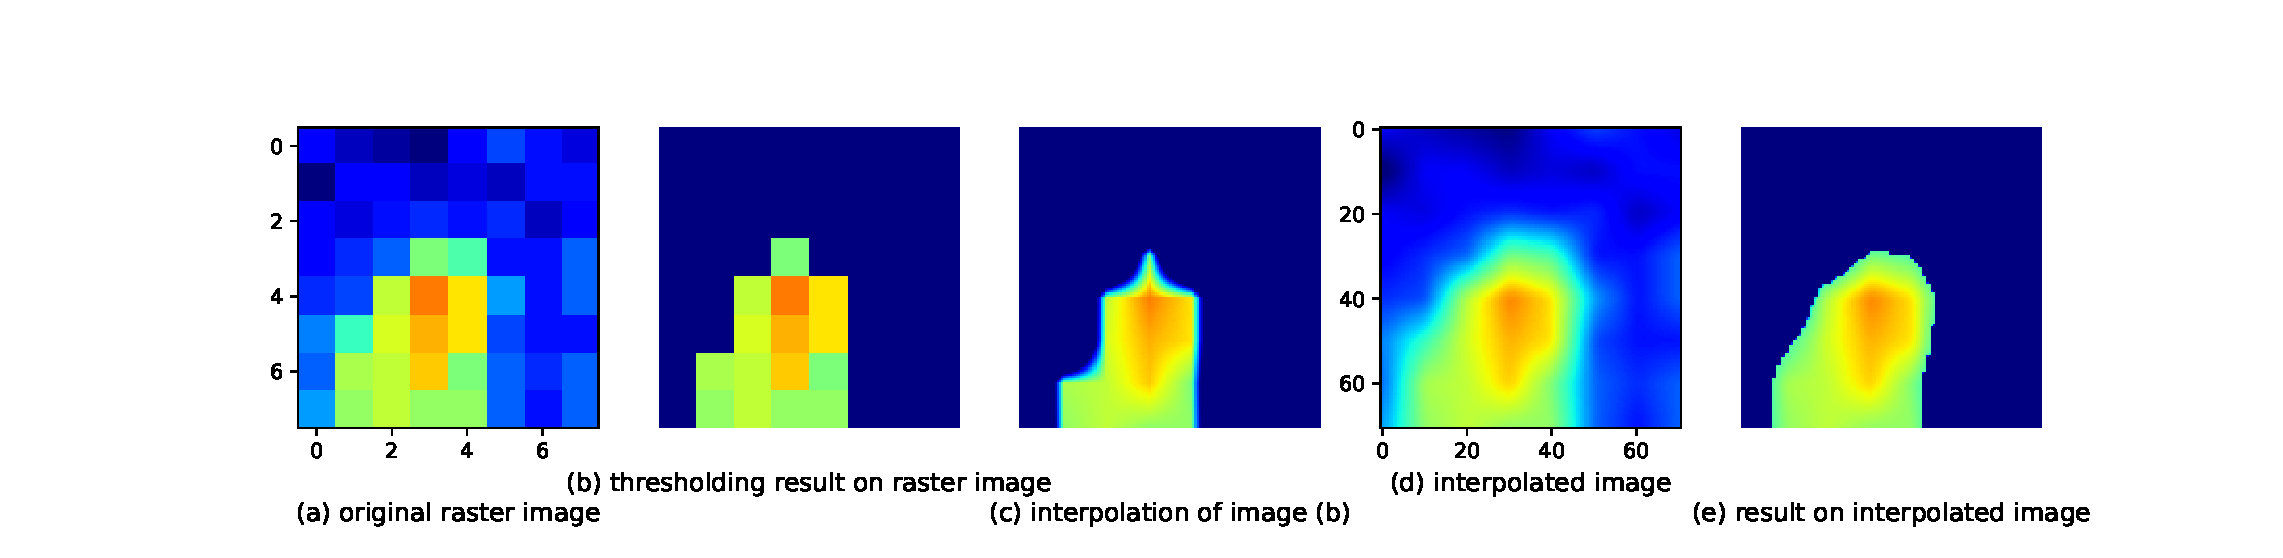
\includegraphics[width=\textwidth]{figures/detect_interpolate.eps}
  \caption{Result given by \autoref{eq:detectionthreshold}, the interpolated image preserves more details after thresholding.}\label{fig:detectioninterpolate}
\end{figure}

\subsection{a spacial filter}
We notice that a single global threshold cannot separate two close objects very well. When two human stand close to each other, the small region between them will have a temperature higher than the room temperature because the pixel value results from a size-weighted average of both objects and background. This effect creates fake active pixels in the binary mask, see the first row in \autoref{fig:detectionspatialfilter}.

Therefore, pixels with hotter pixels nearby should be ignored because they origins from those hotter pixels and do not represent the true heat distribution. Reversely speaking, only those pixels that are hotter than its surrounding, namely local maxima pixels, contain valid information. We use the average filtered image as a spatial filter. After experiments on the collected image frames, a kernel size of 36 is chosen (half of the frame width). The value of every pixel in the filter is calculated by averaging a $36\times36$ neighbourhood surrounding that pixel location in the original image. Afterwards, the original image is compared with the filter pixel-wise, and only those pixels with a value higher than its filter counterpart will be kept. \autoref{fig:detection3d} shows the process in a surface plot, it shows the same image frame from \autoref{fig:detectionspatialfilter}. The threshold calculated from \autoref{eq:detectionthreshold} is applied to the local maxima image. The result is shown in the second row of \autoref{fig:detectionspatialfilter}, it is clear that the bridge connects two objects becomes much narrower. This method outperforms 
\begin{figure}
  \centering
  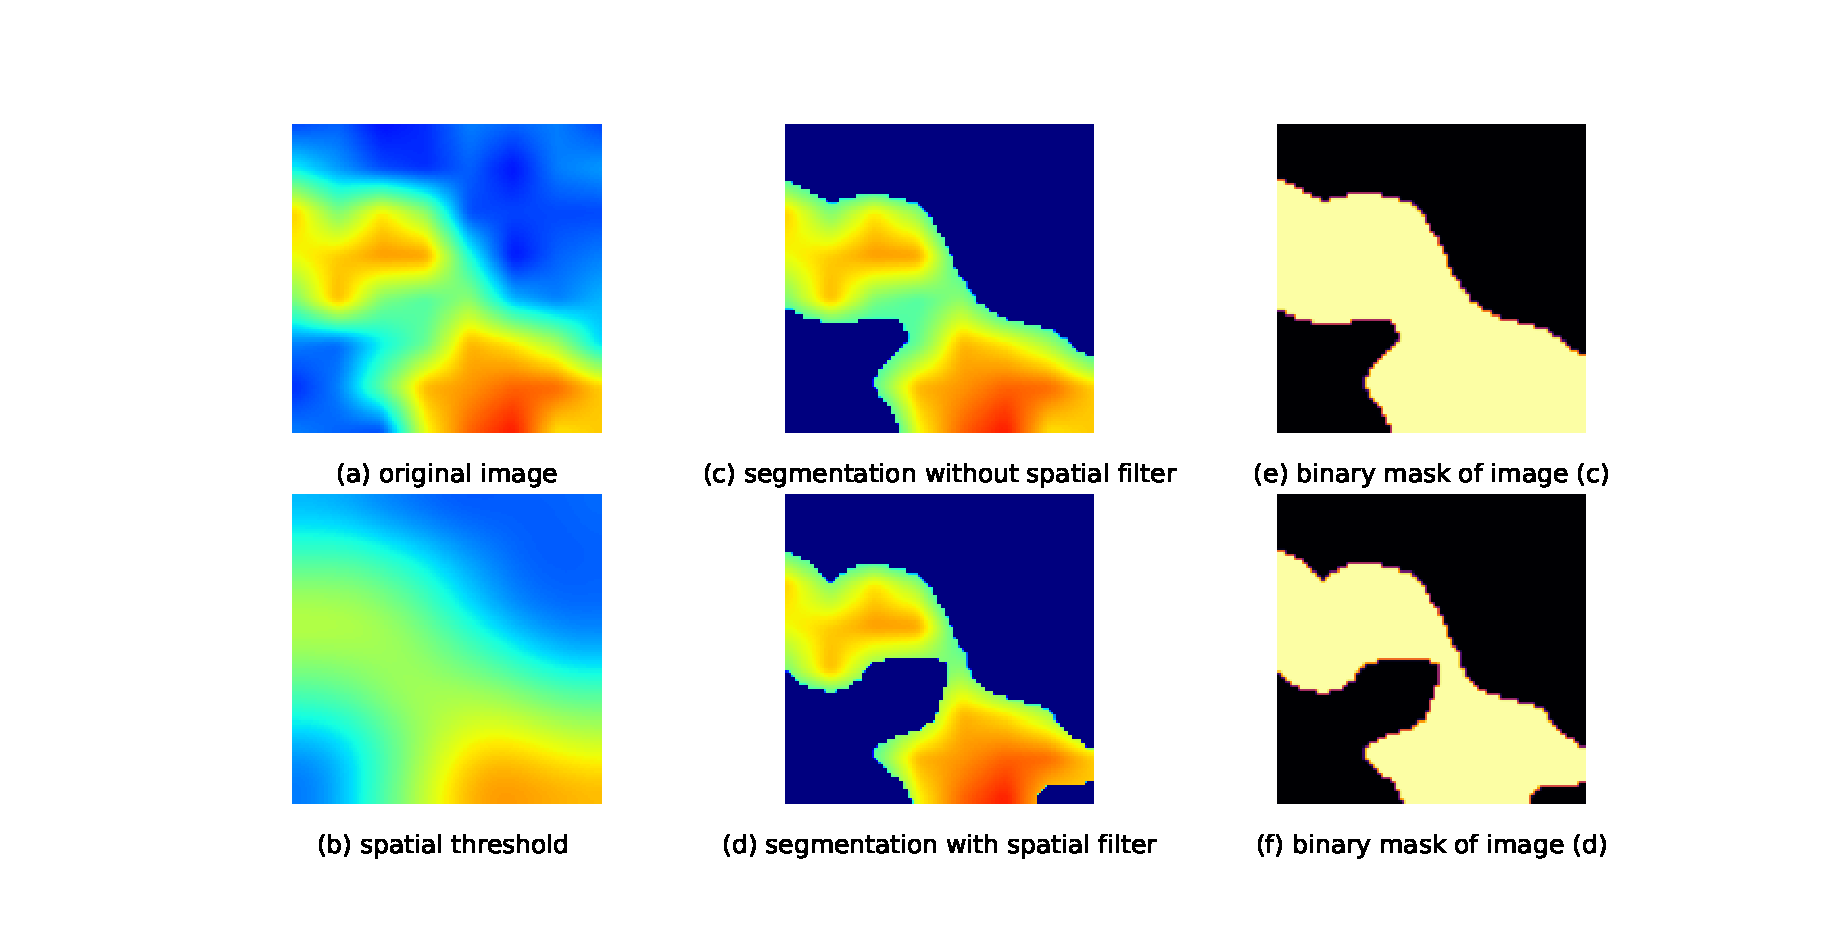
\includegraphics[width=\textwidth]{figures/detect_spatialfilter.eps}
  \caption{After introducing a spatial filter, the region between two objects are no longer marked as occupied.}\label{fig:detectionspatialfilter}
\end{figure}
\begin{figure}
  \centering
  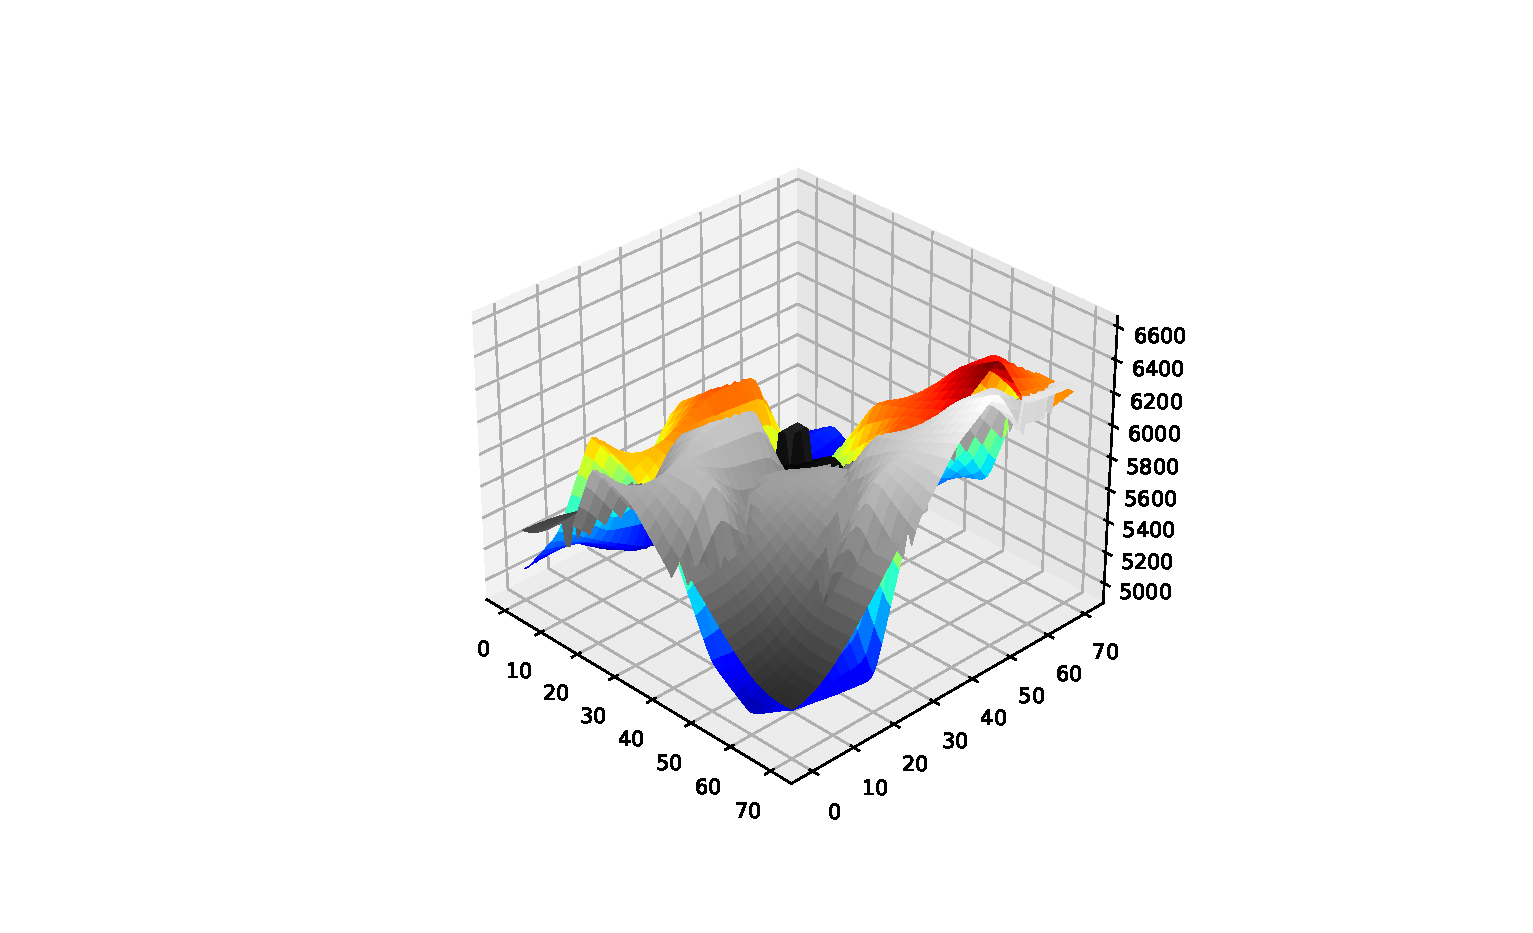
\includegraphics[width=\textwidth]{figures/detect_filterthres.eps}
  \caption{Only those pixels hotter than region average is kept. The gray layer is the average filtered image and the colored layer is the original image.}\label{fig:detection3d}
\end{figure}


\subsection{filling holes}
\section{Feature Extraction}
\section{Human Object Tracking}
\section{Feature Extraction} \label{sec:featureextract}
The binary blob mask of an object contains too much redundant information for the tracking algorithm. As reviewed in \autoref{ch:review}, a binary blob could be represented as a feature vector of the centroid and the size, denoted as \autoref{eq:blobdenote1}, where $C$ is the 2D coordinate of the geometry center and $S$ is the total pixel number of the blob.
\begin{equation}\label{eq:blobdenote1}
  B = \{C,S\}
\end{equation}

This basic representation is sufficient for a single object tracking because the centroid is a unique feature for a blob. However, when two objects overlap and their blob masks merge together, they will be regarded as one single blob and therefore have only one shared centroid. The uniqueness of the centroid no longer holds, and the one-to-one matching relation between an object and its corresponding blob mask is broken.
\autoref{fig:blobmerge} shows an example demonstrating how the merged blobs impede the feature extraction. In the first two frames where two blobs are not merged, their centroids remain unique and transit a small shift from the last frame. The size of the blobs remain similar as the last frame as well. In the third frame, the blobs are merged, their centroids disappear and is replaced with a single centroid at the center of two blobs. Viewing the extracted feature only, we may only conclude that there is one blob with twice the size as before. Furthermore, the location of the centroid jumps abruptly, not close to either centroids in the last frame. In the fifth frame, the blobs are again separated. An abrupt change in centroid position takes place again.

Since the tracker match objects with its nearest neighbour in the last frame, a distance that is too long will break the matching. Even if the blobs are successfully matched, a shared centroid will bring ambiguity to the label assignment. Labels may be exchanged between two objects after splitting.
\begin{figure}
  \centering
  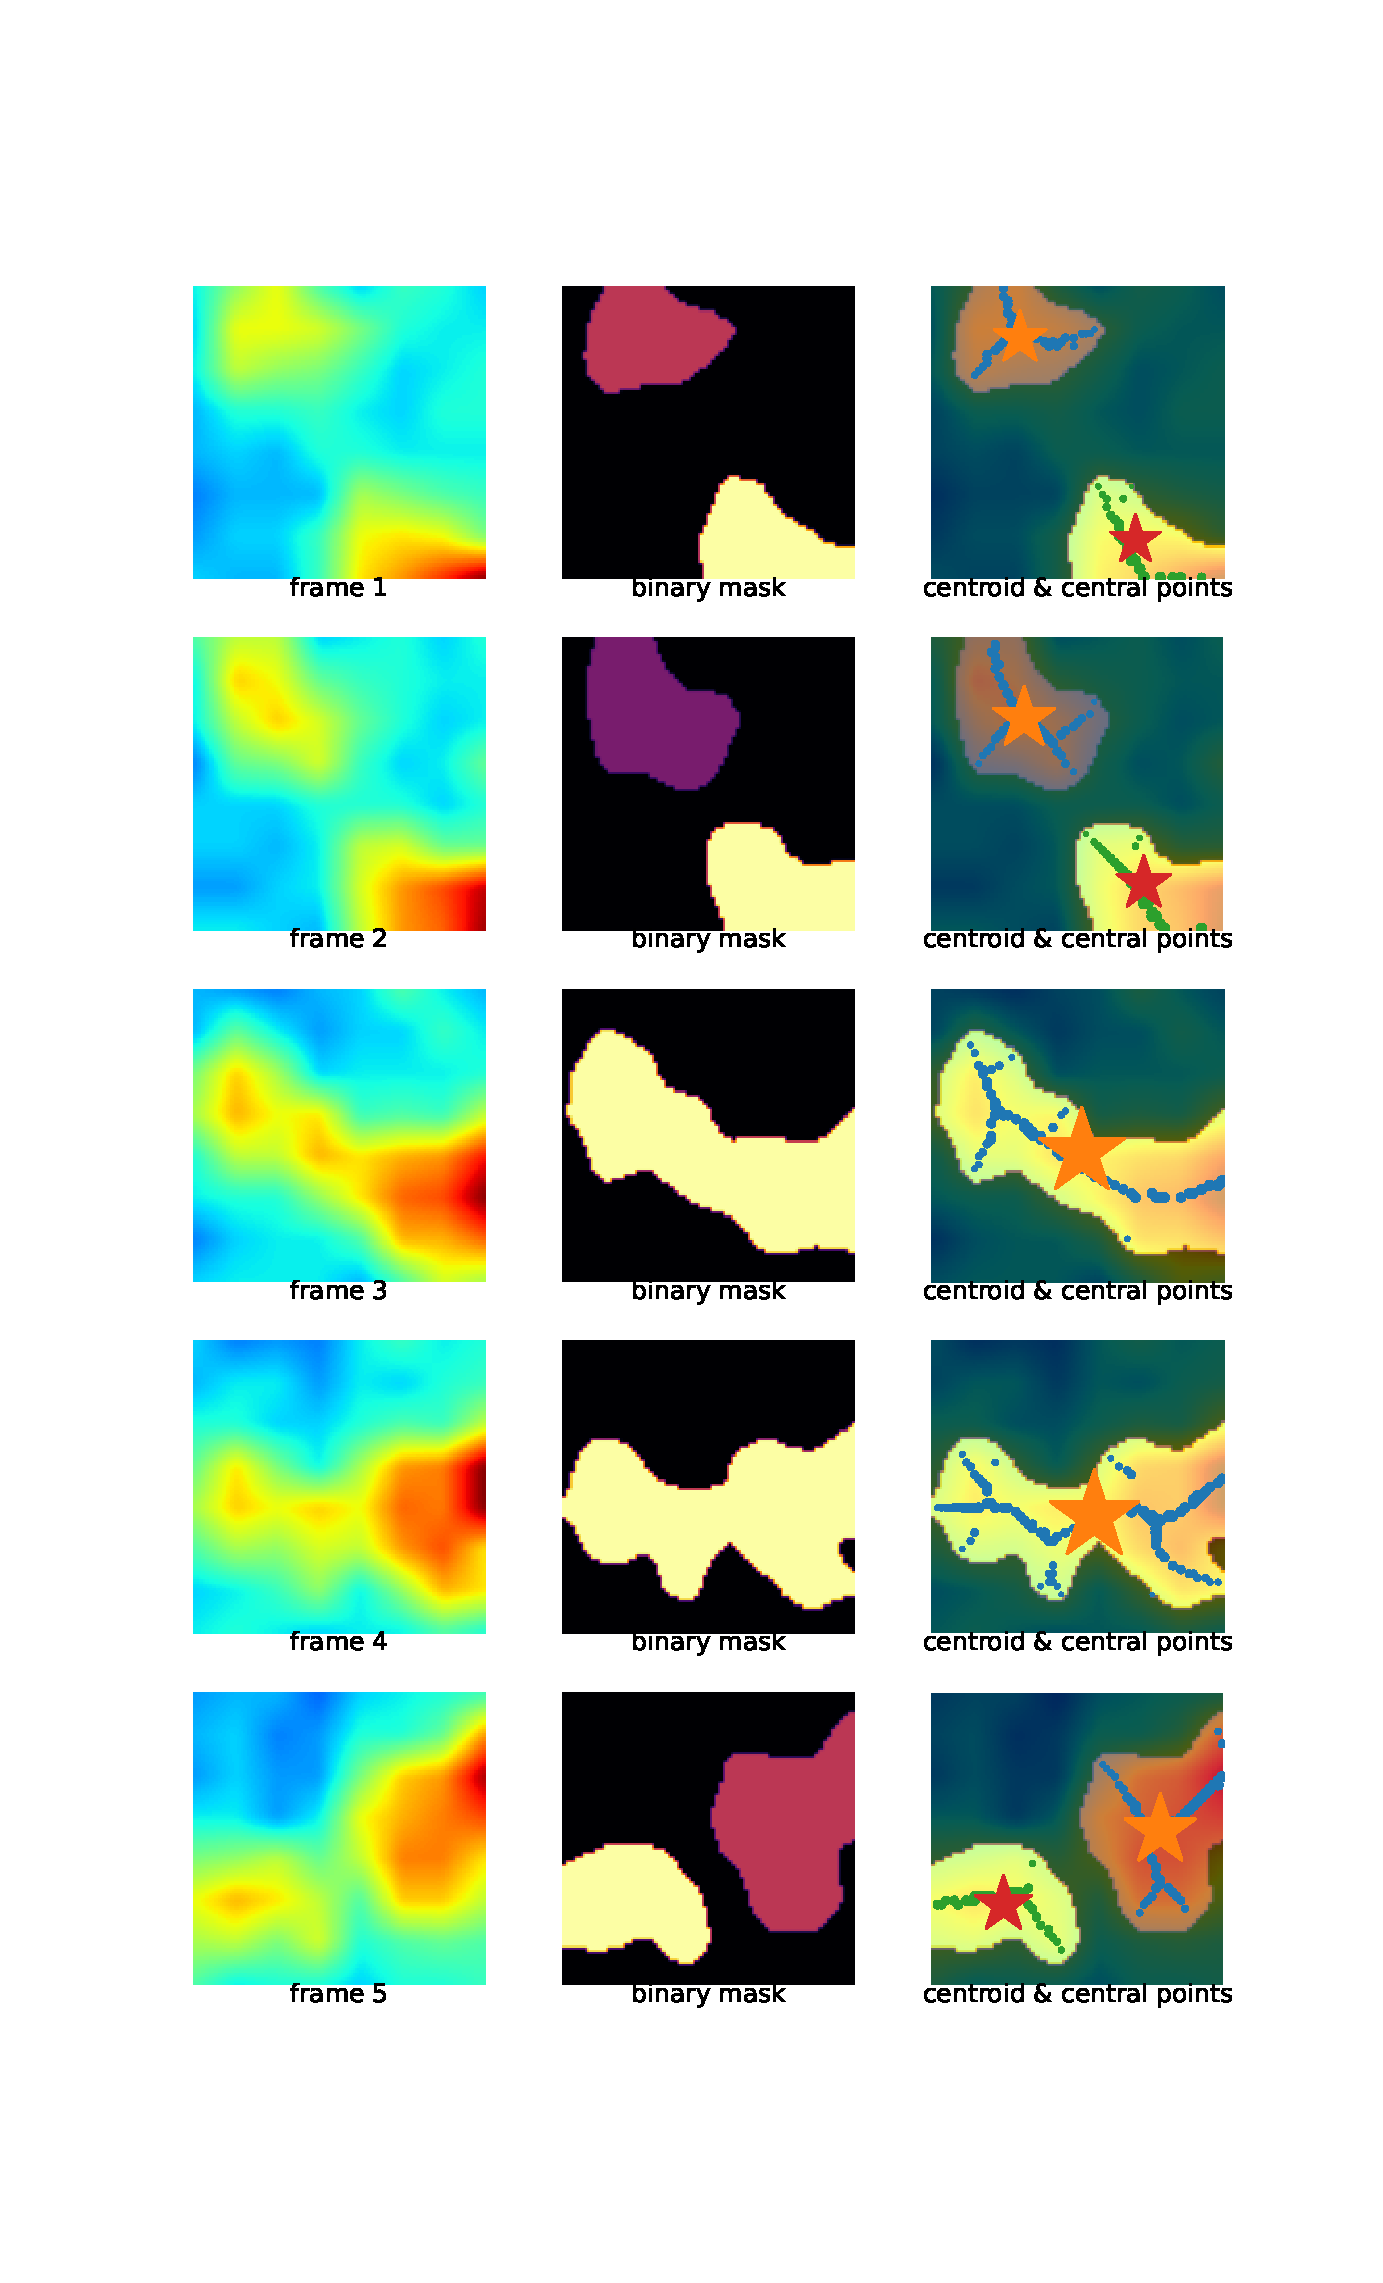
\includegraphics[width=0.6\textwidth]{figures/blobmerge.eps}
  \caption{An example frame sequence showing the blob merging issue. Left column is the interpolated image, middle column is the blob masks and right column shows the extracted feature. The star symbol represents the centroid location and the size of the start represents the size of the blob. Other round dots scattered inside the blob represent central points.}\label{fig:blobmerge}
\end{figure}

We follow the research of \cite{sharma2012blob}, adding ``central points'' as addition feature for blob representation. Central points of a blob are those points that are far away from the background, they can be found out by picking local maxima in a distance transform of the blob mask.
\subsection{introduction of distance transform}
A distance transform of a binary image labels every pixel of the image by the distance between that pixel and the nearest background pixel \cite{bailey2004efficient}, which could be denoted as \autoref{eq:distancetransform}.
\begin{equation}\label{eq:distancetransform}
  I_d(x,y) = \left\{\begin{array}{cc}
               0 & I(x,y)\in\{Bg\} \\
               \min\left(\Vert x-x_0,y-y_0\Vert\right),\forall I(x_0,y_0)\in Bg & I(x,y)\in\{Ob\}
             \end{array}\right.
\end{equation}
The $\Vert\cdot\Vert$ symbol is a distance definition, could be $L_1$, $L_2$, $L_{max}$ or any other distance metric. To our concern, the distance is measured in Euclidean metric, namely $\Vert x,y\Vert=\sqrt{x^2+y_2}$.

A precise computation of the Euclidean distance transform is complex. A commonly used approximation is the chamfer distance transform \cite{butt1998optimum}. The chamfer distance transform exploits the fact that the distance between of each pixel to its nearest background pixel depends on the previously computed neighbour. The whole distance transform image could be obtained in two pass, one propagating from the upper-left corner to the lower-right corner and the other reversely.

\begin{table}
  \centering
  \begin{tabular}{|c|c|c|}
    \hline
    % after \\: \hline or \cline{col1-col2} \cline{col3-col4} ...
    b & a & b \\
    a & $x_-$ & - \\
    - & - & - \\
    \hline
  \end{tabular}
  \begin{tabular}{|c|c|c|}
  \hline
    % after \\: \hline or \cline{col1-col2} \cline{col3-col4} ...
    - & - & - \\
    - & $x_+$ & a \\
    b & a & b \\
    \hline
  \end{tabular}
  \caption{Distance increment of two pass respectively for a $3\times3$ window.}\label{tab:chamfertable}
\end{table}

\subsection{local maxima in a distance transform}

\subsection{central points - an informative and stable representation}
Central points preserve most information about the original blob. If the distance value to the background of every central point is preserved, the original blob mask could be approximately recovered from the central points, see \autoref{fig:maskrecover}. In contrary, the shape information is lost when using the centroid representation. Certainly, multiple central points requires more memory space than a single centroid, but the central points representation compresses information efficiently.
 
The cluster of central points looks like the ``spine'' of the original blob.
\begin{figure}
  \centering
  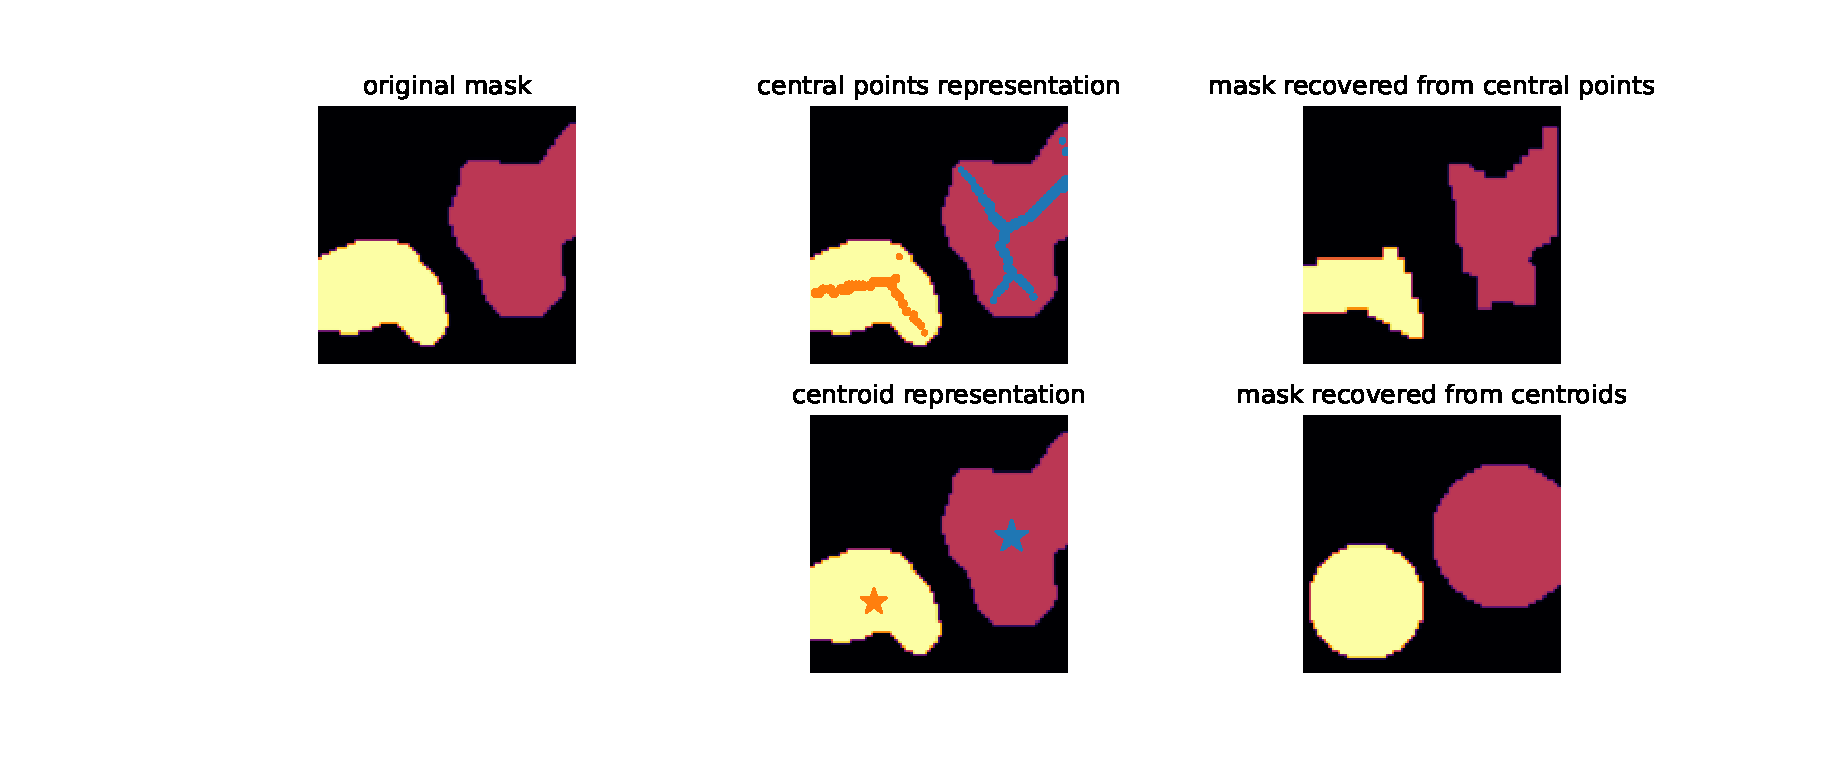
\includegraphics[width=\textwidth]{figures/maskrecover.eps}
  \caption{mask recover}\label{fig:maskrecover}
\end{figure}


\section{Human Object Tracking} \label{sec:track}
After abstracting the blob masks into feature vector representation shown in \autoref{eq:blobdenote2}, the tracking algorithm finally comes into use. To handle the one-to-many relation between blobs and actual objects, we introduce an abstract layer called object layer above the observed blob layer. The tracking algorithm maintains a list of known objects and matches an object with its optimum pair in the blob list given by the feature extractor. Every object consists of the attributes listed in \autoref{tab:objectattributes}.

 Overall speaking, the objective of the tracking layer is to:
\begin{enumerate}
  \item track the blobs by their centroid as much as possible
  \item if step 1 fails, try matching existing object with one of the central points
  \item in step 2, choose the most likely candidate for matching among all central points, considering the previous object location, motion direction as well as speed, as mentioned in \Cref{sec:featureextract}
  \item determine if two blobs actually belong to one previous object, as mentioned in \Cref{sec:detect}
  \item determine if it is an entering/ exiting event by an object's first position and last seen position, as well as modify the room occupancy count
\end{enumerate}

The above listed tracking steps are adapted from \cite{sharma2012blob} for a top-view IR image sequence, and could be further divided into two phases.

In the pairing phase, the location of an object will be updated to the paired blob location with a filter. If an object cannot find a suitable blob pair, it will not be eliminated immediately but continue propagated a few frames with the previous velocity to see if there could be a match on the forward trajectory. This is exactly the virtual track method used by \cite{virtualtrack}.

If there is at least one unmatched blob left in the blob list, the spawn phase is activated. The tracking algorithm first check if the matched blob could be a fraction of a splitted blob. If it is the case, the blob will be merged to the nearby existing object and contribute to the object location update. Finally, if the blob is unlikely to have any relation with existing objects, a new object will be spawned from the blob center.
\begin{table}
  \centering
  \begin{tabular}{|c|l|}
    \hline
    % after \\: \hline or \cline{col1-col2} \cline{col3-col4} ...
    i & unique label \\
    $\vec{x}$ & current position \\
    $\vec{\dot{x}}$ & current velocity \\
    $\vec{x_0}$ & position of first appearance \\
    $t_v$ & number of virtual track propagation \\
    \hline
  \end{tabular}
  \caption{Object attributes for tracking}\label{tab:objectattributes}
\end{table}

\subsection{Matching Step}
The objects and blobs are matched by a distance score based on nearest neighbour rule. By matching, a time disparity between the objects and blobs should be considered. Because the blobs are observed at a time step $t$, but the objects location are updated in the last time step $t-1$. By the time of matching, the objects should have already moved forward. Therefore, the blobs should be matched with the \emph{predicted position} of the objects.

A Kalman filter could be used to store the object states and predict its next state by state transition \cite{mika,virtualtrack}. Since the states in our use case only contain two components (position and velocity), and the second one is the derivative of the first one, an Alpha-Beta filter could be used to simplify the filtering process and cutdown unnecessary computational overhead.

An Alpha-Beta filter resembles the Kalman filter in its nature, combining state transition and observation for state update, but does not vary coefficients dynamically. Denote $\hat{\boldmath{x}}$ as the estimated value, $\boldmath{x}^p$ as the predicted value and $\boldmath{x}^m$ as the measured value, the system state is obtained by the following \autoref{eq:abfilter}.
\begin{equation}\label{eq:abfilter}
  \left\{
  \begin{split}
    & \hat{\boldmath{x}}_n = \boldmath{x_n}^p + \alpha\left(\boldmath{x_n}^m-\boldmath{x_n}^p\right)\\
    & \hat{\boldmath{\dot{x}}}_n = \boldmath{\dot{x}}^p_n + \frac{\beta}{T}\left(\boldmath{x_n}^m-\boldmath{x_n}^p\right)\\
    & \boldmath{x_{n+1}^p} = \hat{\boldmath{x}}_n + T \hat{\boldmath{\dot{x}}}_n\\
    & \boldmath{\dot{x}_{n+1}}^p = \boldmath{\dot{x}_{n}}
  \end{split}
  \right.
\end{equation}

In the first two lines of \autoref{eq:abfilter}, $\alpha$ and $\beta$ are two fixed coefficients that are chosen experimentally. For an camera installed at a height of 2.5m with a FOV of $60^\circ C$, we choose $\alpha=0.75,\ \beta=0.8$. \autoref{fig:trackexample1} demonstrates the smoothen effect of the filter, the estimated trajectory becomes more stable compared to the measured trajectory. More importantly, even though the filter uses fixed coefficients, the prediction usually approximate the actual measurement very well. An exception is when the human moves close to the border, because the human body is only partially detected, the centroid of that partial body stays almost still. The estimated object position will converge quickly to the actual (but wrong) measurement. This behaviour is designed intended so that the tracking could be continued.
\begin{figure}
  \centering
  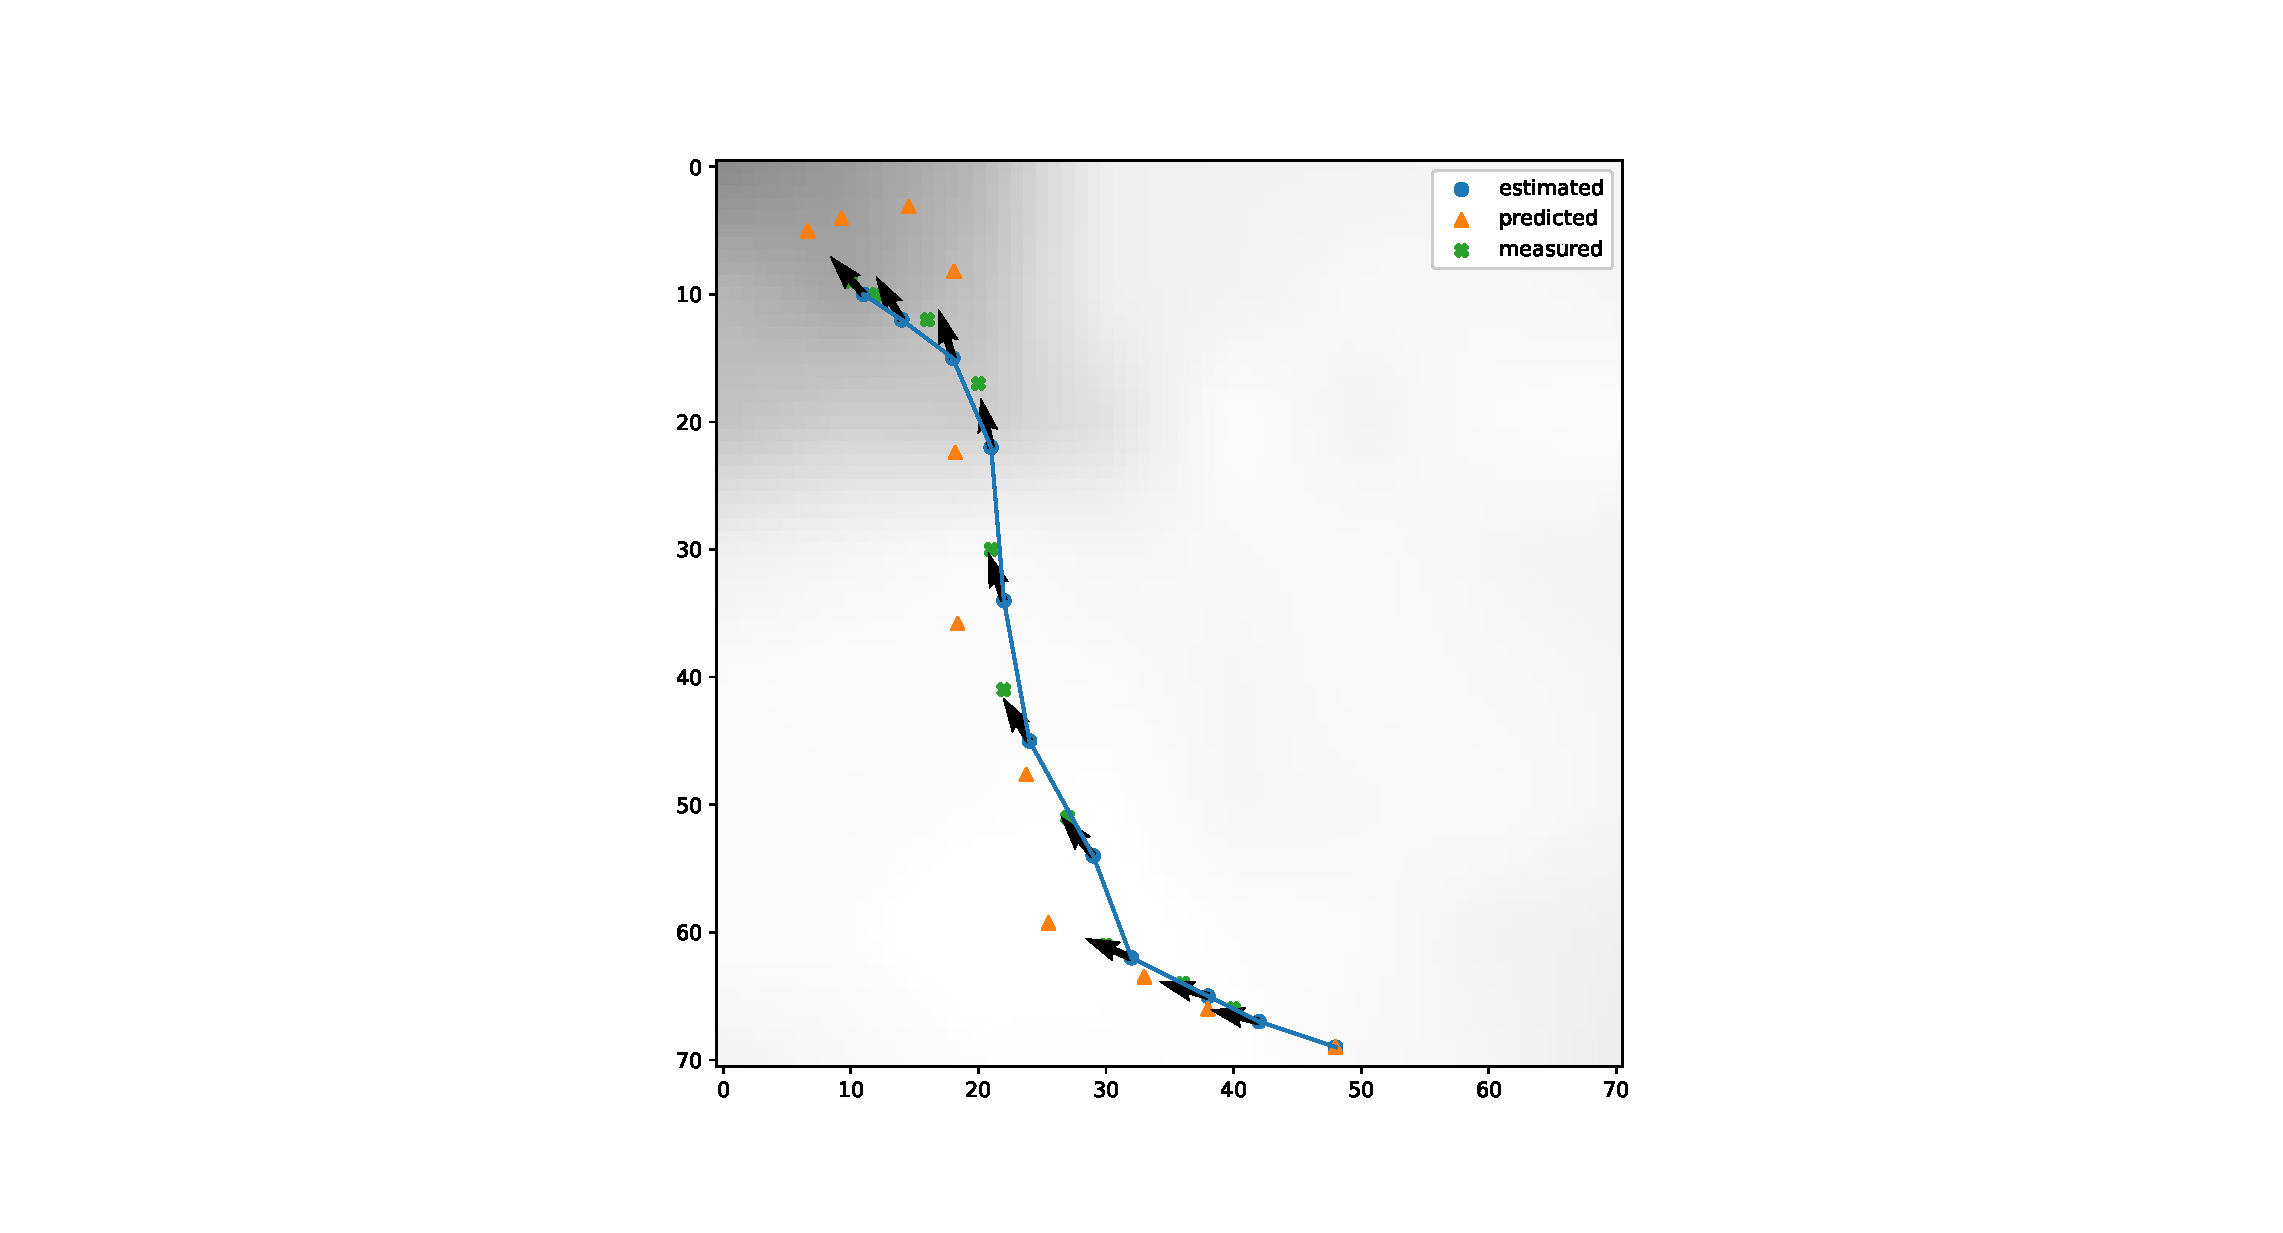
\includegraphics[width=\textwidth]{figures/trackexample1.eps}
  \caption{A track example. The blue dots show the estimated position, the arrow from the blue dot points the velocity direction of the object and the yellow triangle shows the predicted position one time step forward.}\label{fig:trackexample1}
\end{figure}

During the middle stem of the trajectory when the human is fully observed, the predicted position given by the filter significantly simplifies the tracking algorithm. The distance threshold between a blob observation and an object no longer depends on the object velocity, but merely on the prediction deviation and measurement error. Therefore, the distance threshold could be reduced to a low value, which potentially avoids false matching because of a large searching radius.

Moreover, an (relatively) accurate prediction could solve the nearest neighbour issue during central point matching mentioned in \autoref{sec:featureextract}. By central points extraction, several points on the child branch would be inevitably picked to be possible candidates, while the actual blob central must locate on the main branch. Since those points on the child branch are closer to the border and therefore closer to the last estimated object location, they will have a higher chance in pairing if we directly match the last estimated object location with the measurement. However, with one time step forward prediction, the predicted object location will locate approximately on the main branch of the central point representation, and the tracking algorithm will choose a candidate that is closer to the actual object position.

For both centroid matching and central points matching, we chose a distance threshold of 15 pixels. This value was chosen based on the camera installation height and normal walking speed.

\begin{figure}
  \centering
  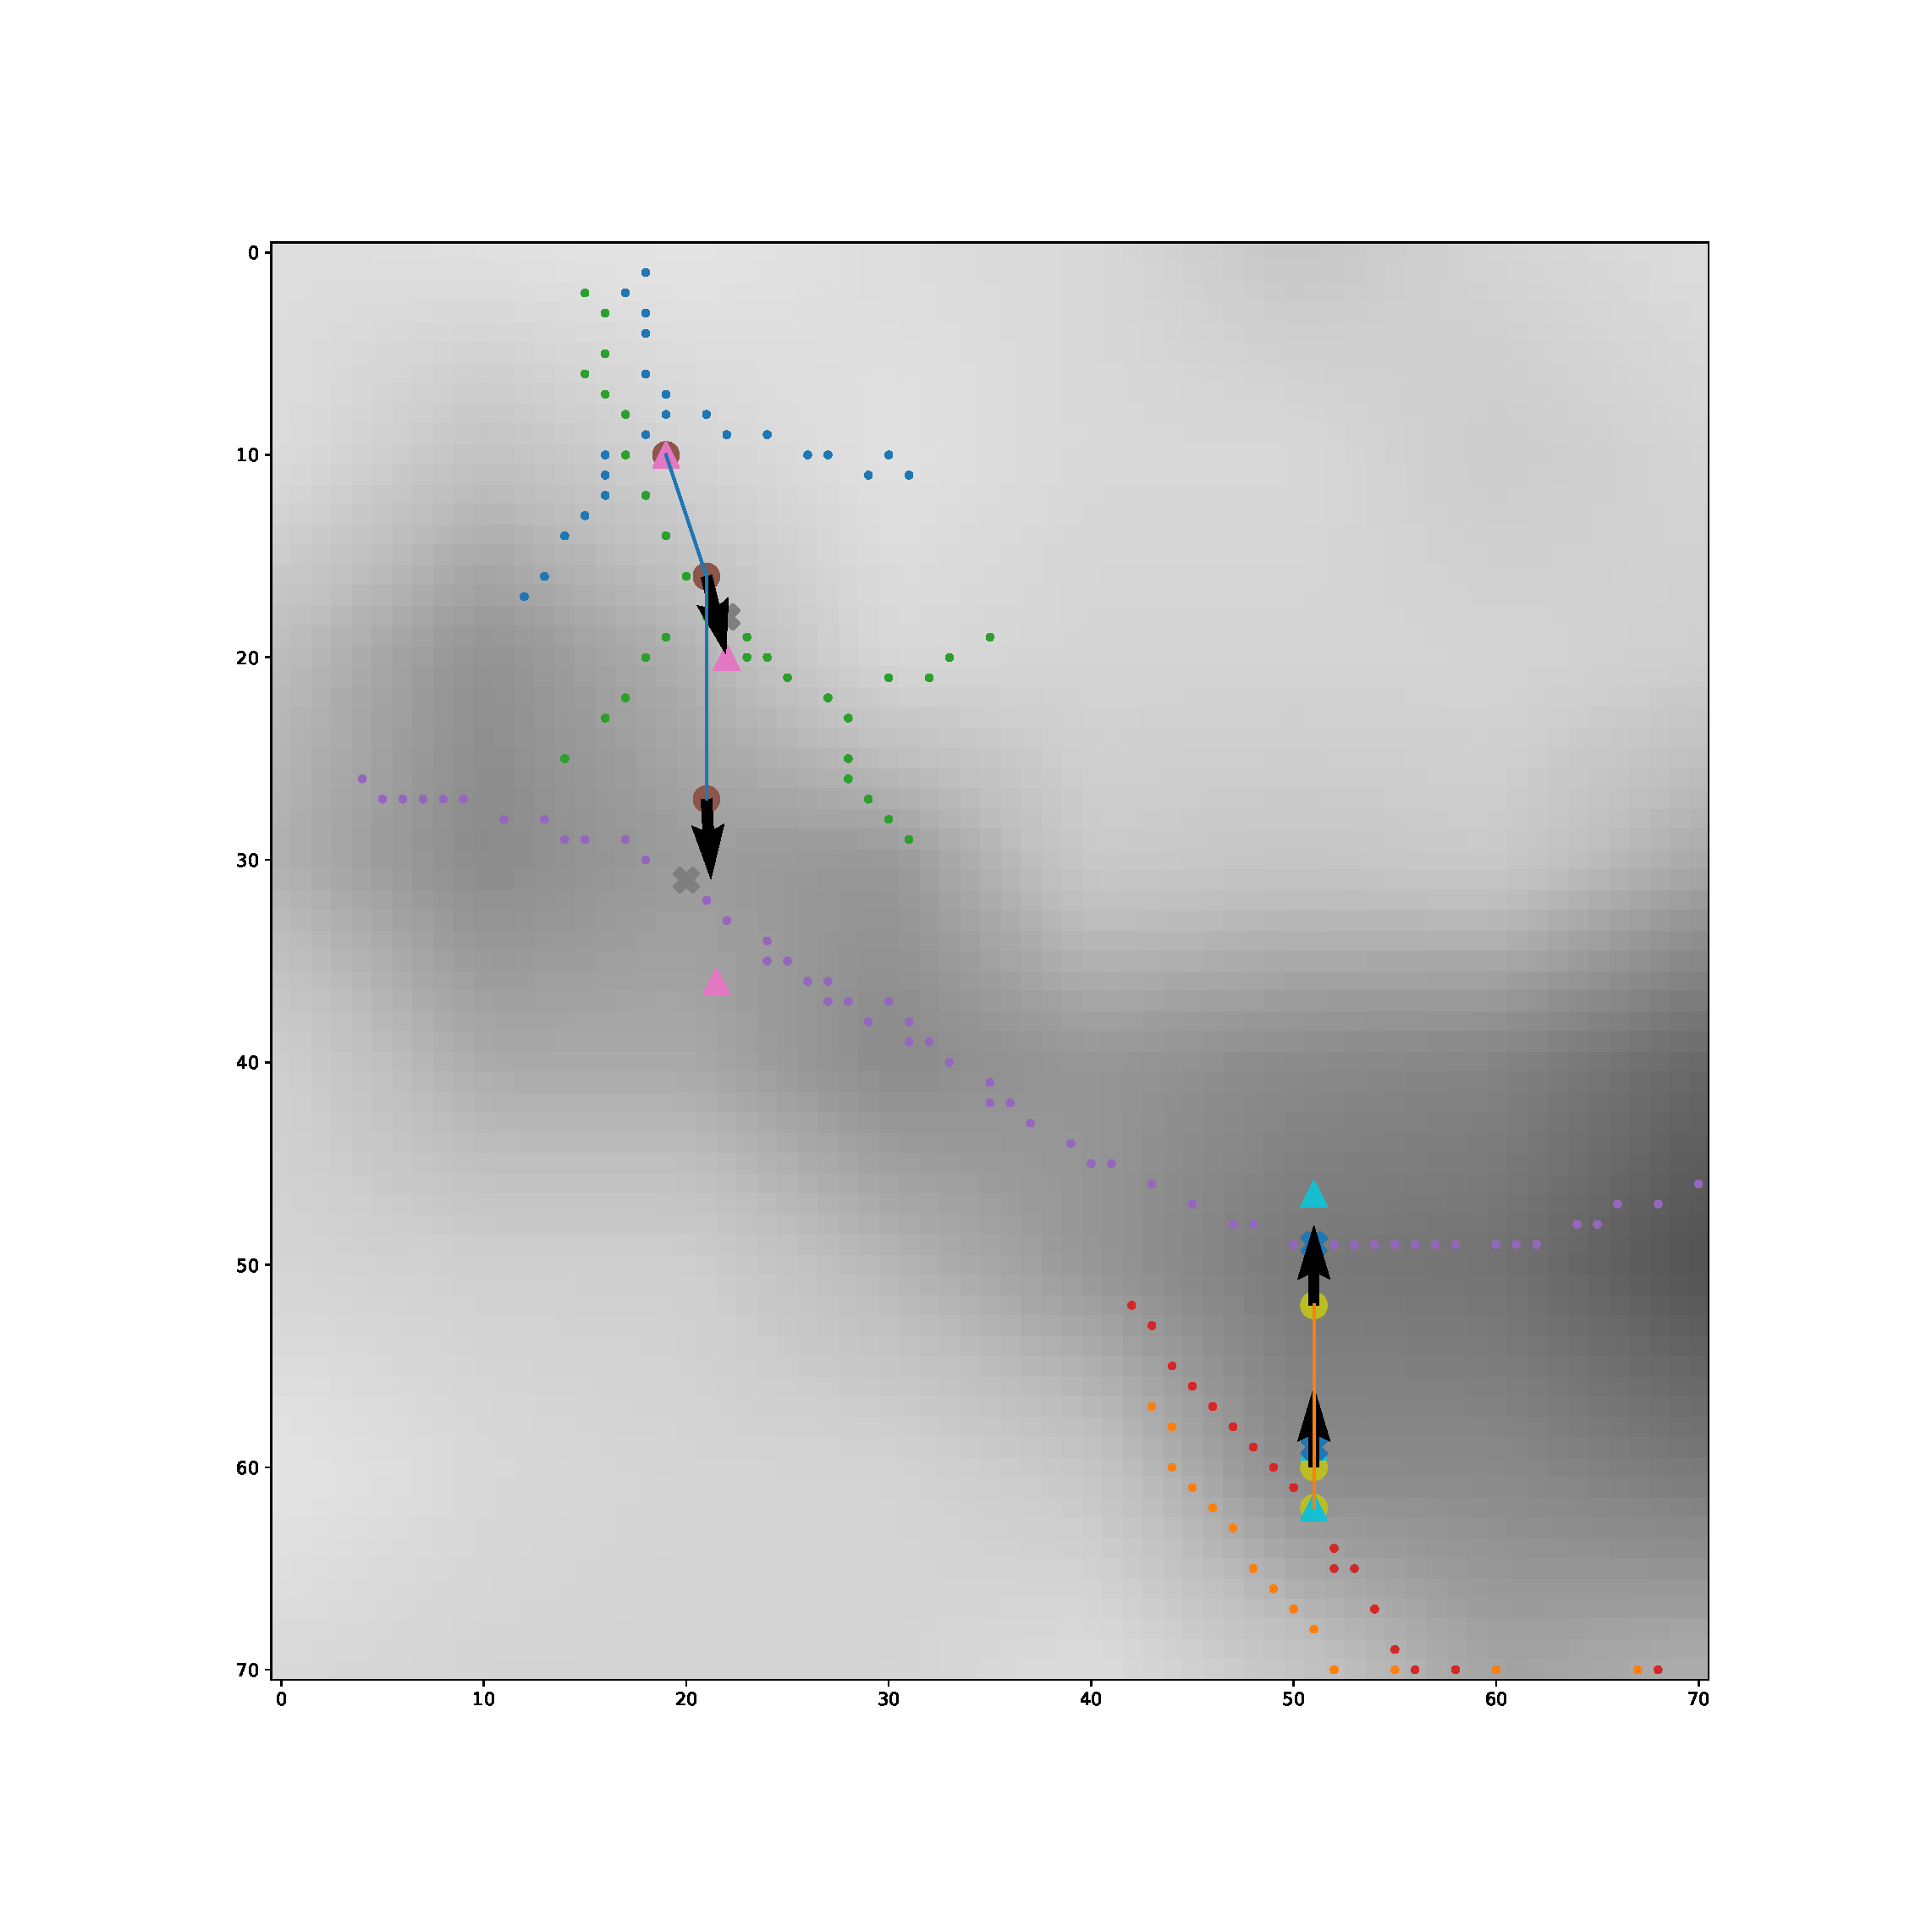
\includegraphics[width=\textwidth]{figures/trackexample2.eps}
  \caption{A track example (same sequence as \autoref{fig:blobmerge}) until two blobs merged and the central point matching is activated. The pixel dots represent the central points. The round markers are the estimated object location, triangle markers are predictions, and cross markers are measurements. The blob contour is omitted for a clear demonstration.}\label{fig:trackexample2}
\end{figure}
\begin{figure}
  \centering
  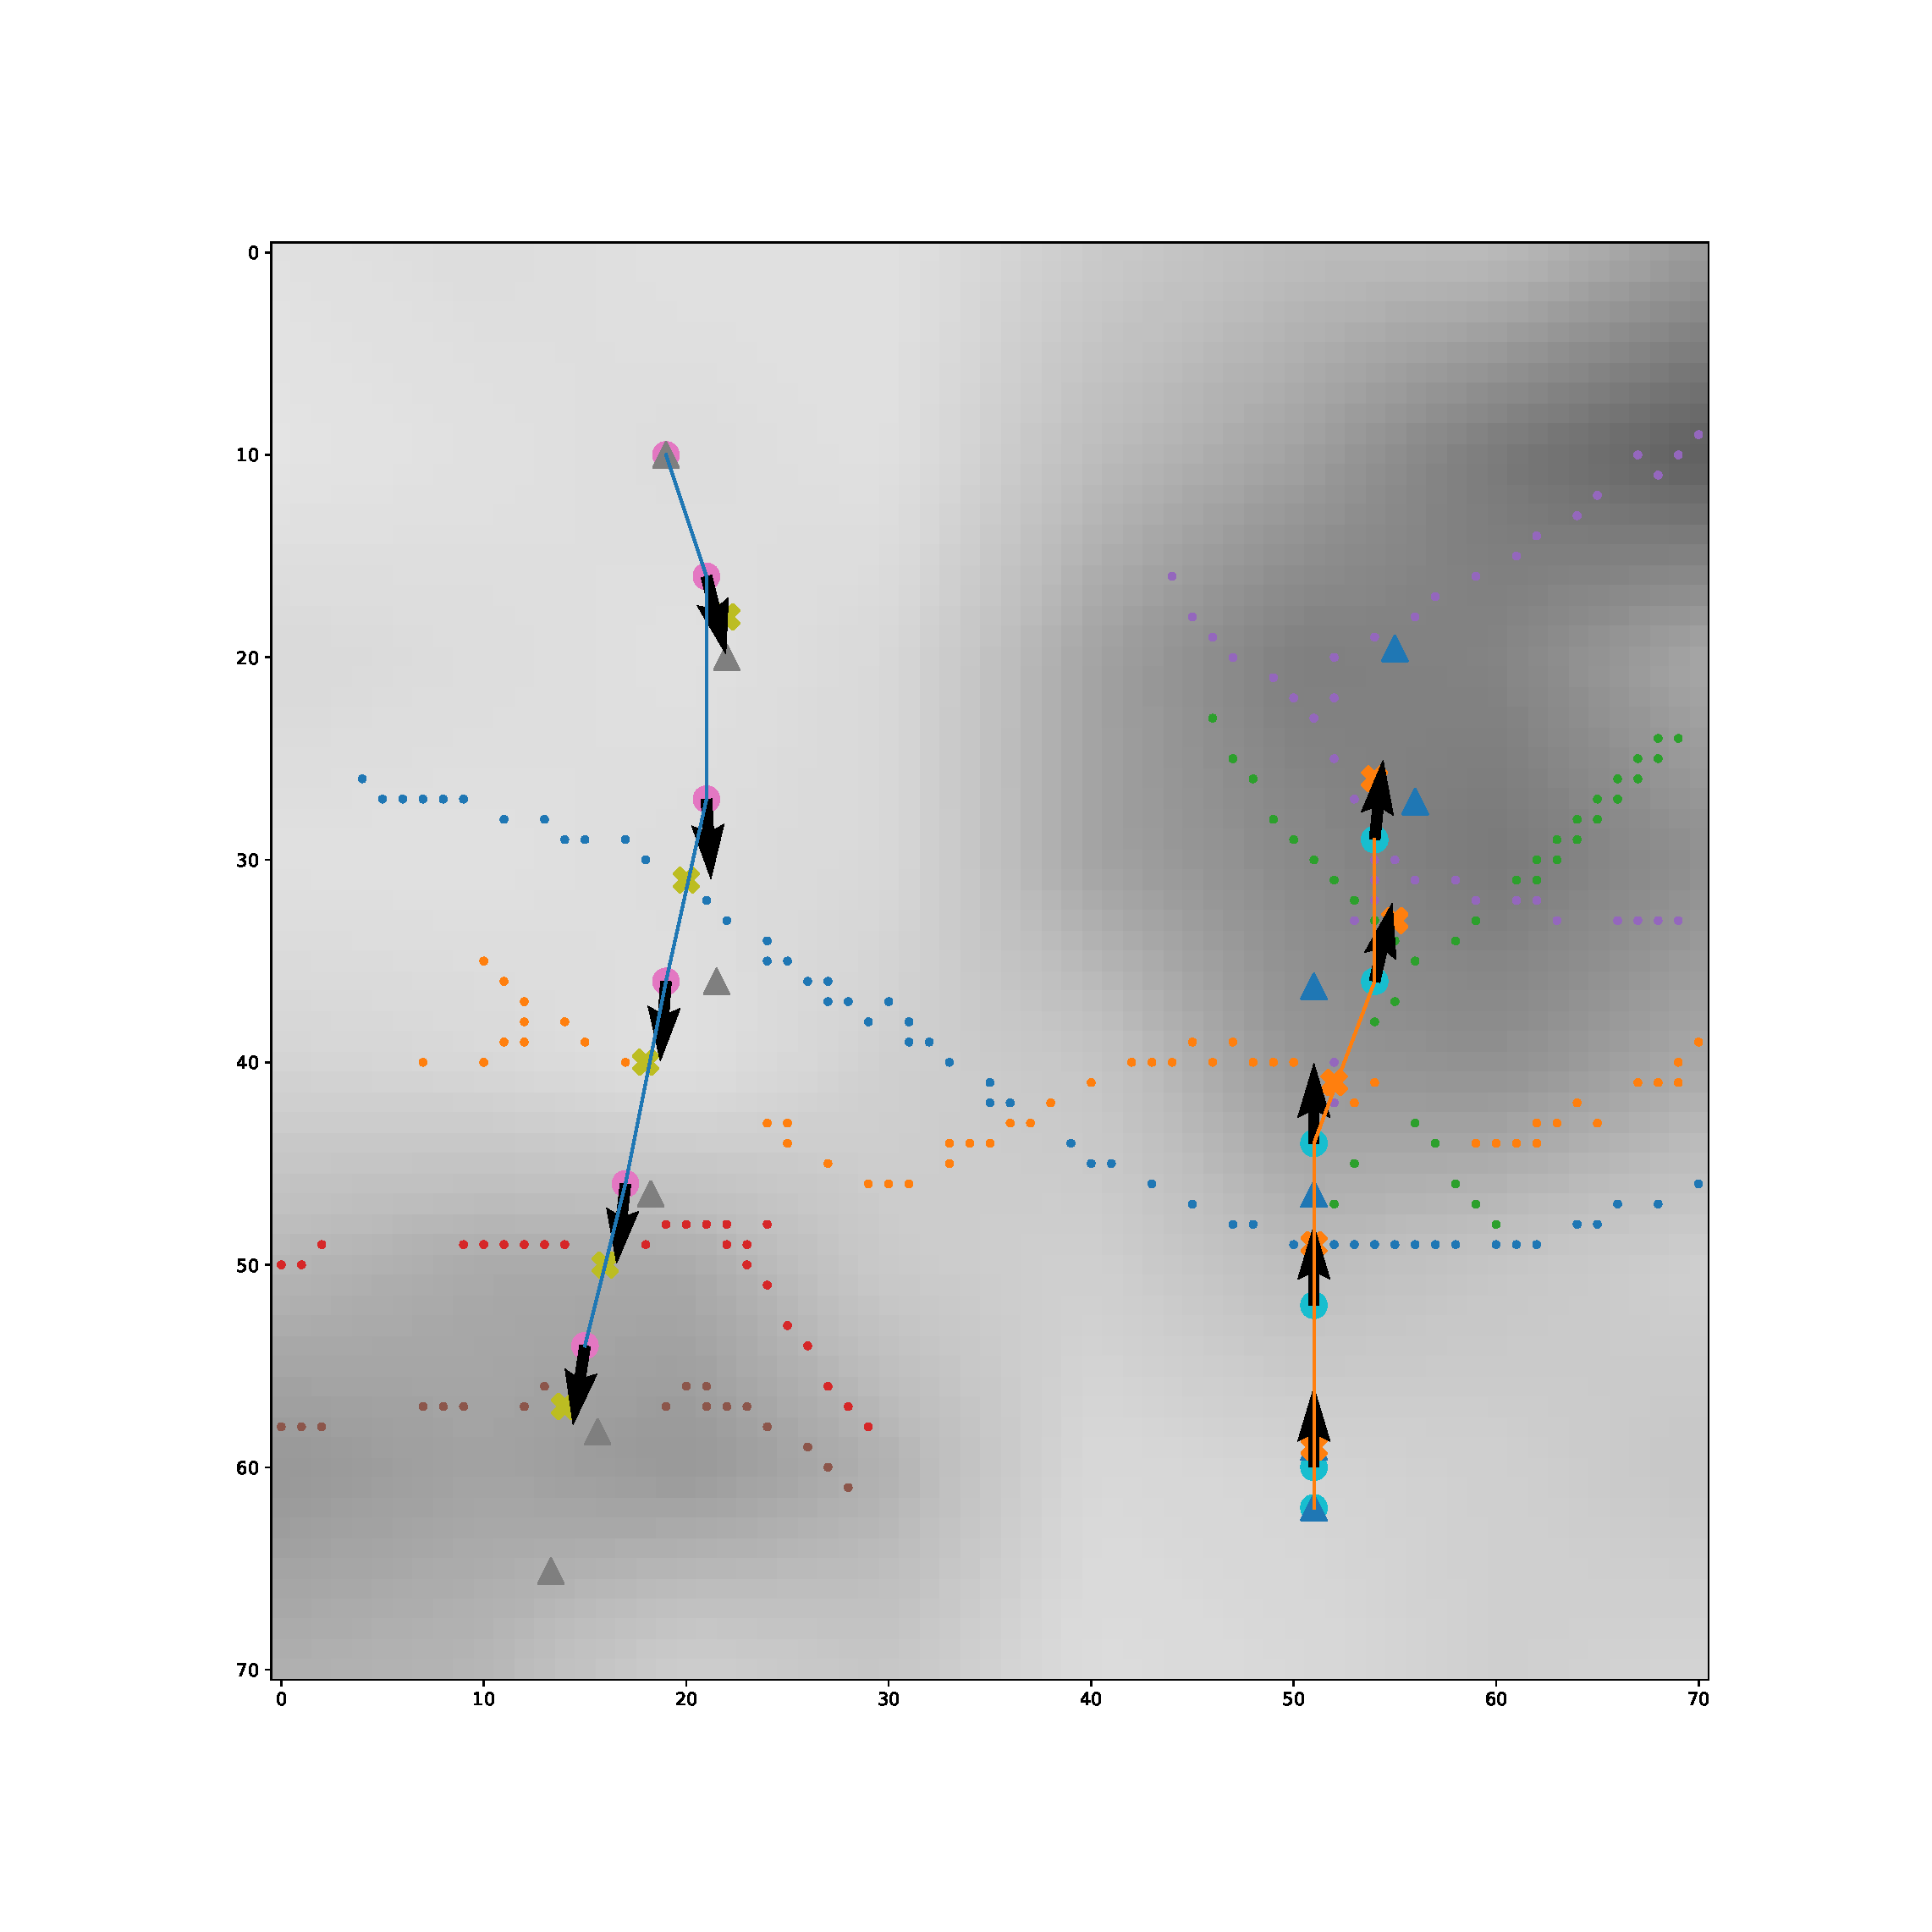
\includegraphics[width=\textwidth]{figures/trackexample2_2.eps}
  \caption{A track example (same sequence as \autoref{fig:blobmerge}, continued from \autoref{fig:trackexample2}) after the merge event. The tracking algorithm successfully handled the merging blobs and continues tracking with centroids.}\label{fig:trackexample2_2}
\end{figure}

\subsection{Virtual Track}
An event-based counting rule is applied to determine the room count value. The object activities are counted after the termination of its trajectory. A count modification of $\pm 1$ will be added to the final count if the object's first and last positions locate on different sides of the doorway middle line.

Beside the matching step based on centroid and central points, we have integrated the virtual track method proposed by \cite{virtualtrack}, though for a different purpose. We notice that sometimes in a frame sequence an object may be missing for a few frames (usually one or two). This could be traced back to the detection layer, where a human body temperature is too low, either because body temperature fluctuation or camera reading noise disturbance; or in the feature extraction layer, when the detected blob contour varies fiercely and generates a distinct central points distribution and causes a matching failure. In either case, a missing frame will immediately terminate the tracking procedure (the tracker believes the object has left the camera view) and output the relative count value by checking if the object has passed the middle line. When the missing frame happens to be the critical one bypass the middle line, the algorithm will output an incorrect relative count value: the frame sequence is separated into two individual sequences, in the first sequence an object appears on one side of the doorway, moving towards the other side and disappears before it reaches the middle line, in the second sequence another object appears from nowhere on the other side of the middle line and moves until it leaves the camera view. In both sequences, neither object has passed the middle line therefore no count is made.

To increase the robustness of our algorithm, an objected is not deleted immediately after a matching failure. Instead its location will be propagated further with previous position and velocity, which is basically a prediction with a larger time step. For the following a few frames, we try matching the predicted location with a blob. If the object is missed for just one frame, this method works very well. \autoref{fig:trackexample3} shows an example where one object is missed out for one frame because it is merged with a hotter object.
\begin{figure}
  \centering
  \includegraphics[width=\textwidth]{figures/trackexample3.eps}
  \caption{Virtual track propagation example (same sequence as \autoref{fig:blobmerge}), the red circle circumscribes the further transited object based on previous location and velocity. The central points are extracted with the percentage maxima distance threshold to deliberately create a detection failure. }\label{fig:trackexample3}
\end{figure}

The virtual track of an object will be created whenever an object does not find a blob to match, even when it leave the camera view. This is mainly for the ease of programm design. When an object normally leaves the camera view, its prediction of several time steps afterwards would locate out of the frame boundary, therefore it will not be incorrectly matched with a newly entered object. However, the virtual track method could only correctly predict the object location when its velocity component is non-zero. When the missing frame in a sequence happens to be the second frame, the prediction would be exactly the same as the initial position. Moreover, because the filter used for object state update, the object would only obtain a velocity component gradually. At the first few frames the object velocity has not yet converge to the actual velocity. And usually an object would only appear in the camera for about 10 frames. Therefore, the virtual track method is only meaningful in the middle section of the trajectory. This is part of the reason why we separate the entire camera view into two regions instead of three, for instance \cite{mika}, to obtain a more noise-tolerant tracking system. We choose a maxima virtual track life time to be two frames, if an object is not detected for more than two frames, it is considered a malfunction in the detection layer.

\subsection{Blob registration}
The tracking algorithm needs to solve the splitted blob issue caused by hair isolation mentioned in \Cref{sec:detect}. A blob observation would be considered ``paired'' if it has been used to update at least one object. Otherwise it could be a new object entering the camera view. When the binary blob of an object was split into two blobs, only one of them could be matched with the corresponding object. The additional blob strongly interfere the matching procedure and could create an object that should not exist. We follow the idea of \citeauthor{sharma2012blob} \cite{sharma2012blob}, to check if a small blob could be a fraction of a previous large blob before spawning a new object from it.

The most important registration criterium is the size of the object. If a blob has splitted and part of it is used to update the object, there will be an abrupt size decay. For any unmatched blob, we check if there is a nearby object whose size just shrunk. If the size of the unmatched blob could compensate the decreased size, it is regarded as part of the object. The size of the object would be updated to the summation of two blobs' size, and the position of the object would be updated to the size-weighted average of two blobs' position.

\chapter{Performance Evaluation} \label{ch:evaluation}
\section{Evaluation in Controlled Environment}
The counting device was firstly mounted at a household doorframe to test its accuracy. The mounting height was about 2 meters and the ambient temperature was around $24^\circ C$. In a 40 minutes test, a test person was asked to enter and exit the room continuously for 100 times. The user interface shown in \autoref{fig:noderedui} was turned on in a smartphone so that the test person can read the algorithm output immediately.

The algorithm detects 94 enter events correctly and 97 exit events correctly. And it has successfully handled multiple-human events, such as sequential entering and passing in opposite directions.
\section{Evaluation in Uncontrolled Environment}
The counting device has also been attached to the ceiling of the main entrance in our faculty department to evaluate its performance in real situations. The mounting height was a little higher than the previous experiment, at about 3 meters. The device has operated for two weeks around the clock, except for the first 2 days in the second week because of a local network update. The device transmits the counting result of the proposed algorithm as well as the actual infrared image for later annotation. By this way, we have collected a valid dataset of 8 days in total. The evaluation time slot begins from 8:00 in the morning and ends at 20:00.

The ground truth is annotated by manually iterating through all received images. For ease of examination, the device has only transmitted images when there are three pixels hotter than ambient temperature. Usually, the image transmission begins when a human enters the camera FOV and terminates when the human leaves. We regard each video sequence as one individual event (or two closely happening events). A timestamp was attached to each video sequence to indicate the time of that event. By this way, the number of images to be reviewed is reduced from several hundreds of thousands to a moderate number of around one thousand.

The manual ground truth annotation can only locate the time of event occurrence to minutes. However, the counting algorithm outputs an accurate millisecond timestamp when the count changes. This time disparity in timestamp has caused difficulty in matching the ground truth and the algorithm output with automatic tools. Therefore the accuracy evaluation is carried out visually. For every ground truth enter or exit event, it is checked if the counting algorithm outputs a correct result (+1 for entering and -1 for exiting) in the nearby 30 seconds. If this is the case we add one to the correct counting category otherwise to the wrong counting category. A false detection, when no event is observed in the ground truth video sequence but the algorithm outputs a non-zero value, also falls into the wrong counting category. See \autoref{fig:ESKibana} for example, the event around 12:00 is a false detection and the event around 14:00 is a wrong counting, both will increase the number of ``wrong counting'' by one.

We have also picked out those events which involve multiple humans entering or exiting simultaneously and evaluated them separately. For such events, correct counting consists of the correct movement direction as well as the correct counting number. The counting of a multiple-human event is only regarded correct when the algorithm outputs the exact human number as observed in the ground truth. Take \autoref{fig:ESKibana} as an example, the long green bar plots around 11:20 and 16:00 are two correctly counted multiple-human events, and the events around 13:00 and 14:00 are wrong counting. Note that sometimes the algorithm outputs ``+2'' and two single entering events are observed at that time point, we regard such events as correctly counted.

The dataset statics are shown in \autoref{tab:eva_data}, all data are grouped in 2-hour time ranges. We have finally counted 222 correct and 50 wrong outputs in single human events, which amounts to an accuracy of 81.6\%. There have also been 10 correct and 6 wrong outputs in multiple-human events, which amounts to an accuracy of 62.5\%. The overall accuracy is around 80\%.

\begin{table}[]
\small
\begin{tabular}{l|ll|ll|l|ll|ll|}
\cline{2-5} \cline{7-10}
                            & \multicolumn{2}{l|}{single-human event} & \multicolumn{2}{l|}{multi-humans event} &       & \multicolumn{2}{l|}{single-human event} & \multicolumn{2}{l|}{multi-humans event} \\ \hline
\multicolumn{1}{|l|}{Day1}  & correct             & wrong             & correct             & wrong             & Day2  & correct             & wrong             & correct             & wrong             \\ \hline
\multicolumn{1}{|l|}{8:00}  & -                   & -                 & -                   & -                 & 8:00  & 5                   & 1                 & -                   & -                 \\
\multicolumn{1}{|l|}{10:00} & -                   & -                 & -                   & -                 & 10:00 & 10                  & 4                 & 1                   & 0                 \\
\multicolumn{1}{|l|}{12:00} & 9                   & 1                 & -                   & -                 & 12:00 & 11                  & 1                 & 0                   & 2                 \\
\multicolumn{1}{|l|}{14:00} & 4                   & 0                 & 1                   & 0                 & 14:00 & 24                  & 5                 & 1                   & 1                 \\
\multicolumn{1}{|l|}{16:00} & 5                   & 0                 & 0                   & 1                 & 16:00 & 9                   & -                 & -                   & -                 \\
\multicolumn{1}{|l|}{18:00} & 5                   & 1                 & -                   & -                 & 18:00 & -                   & -                 & -                   & -                 \\ \hline
\multicolumn{1}{|l|}{Day3}  & correct             & wrong             & correct             & wrong             & Day4  & correct             & wrong             & correct             & wrong             \\ \hline
\multicolumn{1}{|l|}{8:00}  & 8                   & 2                 & -                   & -                 & 8:00  & -                   & -                 & -                   & -                 \\
\multicolumn{1}{|l|}{10:00} & 5                   & 1                 & -                   & -                 & 10:00 & -                   & 1                 & -                   & -                 \\
\multicolumn{1}{|l|}{12:00} & 0                   & 1                 & 0                   & 1                 & 12:00 & 1                   & 1                 & -                   & -                 \\
\multicolumn{1}{|l|}{14:00} & 2                   & 0                 & 2                   & 0                 & 14:00 & 5                   & 2                 & -                   & -                 \\
\multicolumn{1}{|l|}{16:00} & 2                   & 0                 & -                   & -                 & 16:00 & 2                   & 1                 & 3                   & 0                 \\
\multicolumn{1}{|l|}{18:00} & -                   & -                 & -                   & -                 & 18:00 & -                   & -                 & -                   & -                 \\ \hline
\multicolumn{1}{|l|}{Day5}  & correct             & wrong             & correct             & wrong             & Day6  & correct             & wrong             & correct             & wrong             \\ \hline
\multicolumn{1}{|l|}{8:00}  & -                   & -                 & -                   & -                 & 8:00  & 7                   & 1                 & -                   & -                 \\
\multicolumn{1}{|l|}{10:00} & 0                   & 3                 & 0                   & 1                 & 10:00 & 1                   & 0                 & -                   & -                 \\
\multicolumn{1}{|l|}{12:00} & 7                   & 4                 & -                   & -                 & 12:00 & 6                   & 1                 & -                   & -                 \\
\multicolumn{1}{|l|}{14:00} & 7                   & 0                 & 1                   & 0                 & 14:00 & 8                   & 1                 & -                   & -                 \\
\multicolumn{1}{|l|}{16:00} & -                   & -                 & -                   & -                 & 16:00 & 4                   & 0                 & -                   & -                 \\
\multicolumn{1}{|l|}{18:00} & -                   & -                 & -                   & -                 & 18:00 & 3                   & 1                 & -                   & -                 \\ \hline
\multicolumn{1}{|l|}{Day7}  & correct             & wrong             & correct             & wrong             & Day8  & correct             & wrong             & correct             & wrong             \\ \hline
\multicolumn{1}{|l|}{8:00}  & -                   & -                 & -                   & -                 & 8:00  & 2                   & 0                 & -                   & -                 \\
\multicolumn{1}{|l|}{10:00} & 1                   & 3                 & -                   & -                 & 10:00 & 2                   & 0                 & -                   & -                 \\
\multicolumn{1}{|l|}{12:00} & 9                   & 1                 & -                   & -                 & 12:00 & 5                   & 1                 & -                   & -                 \\
\multicolumn{1}{|l|}{14:00} & 9                   & 2                 & 1                   & 0                 & 14:00 & 13                  & 3                 & -                   & -                 \\
\multicolumn{1}{|l|}{16:00} & 8                   & 3                 & -                   & -                 & 16:00 & 18                  & 3                 & -                   & -                 \\
\multicolumn{1}{|l|}{18:00} & 4                   & 1                 & -                   & -                 & 18:00 & 1                   & 0                 & -                   & -                 \\ \hline
\end{tabular}
\caption{Dataset statistics. The "-" symbol means entry is not applicable.}\label{tab:eva_data}
\end{table}

\section{Discussion}
To investigate what has caused the performance drop in the real situation, the observed possible issues have been categorized into five classes. And they are:
\begin{enumerate}
  \item Not detected: when a hot object is observed in the ground truth but the algorithm does not respond at all.
  \item Noise: when there is only random temperature fluctuation in the scene but the algorithm reports an object entering or leaving.
  \item Long sequence: when a human stands beneath the camera for a long period (several minutes).
  \item Heat disturbance: when the background temperature is not homogenous in the whole scene, for example, half of the FOV monitoring the sunny side of a doorway has a higher temperature.
  \item Missing frame: when somehow a few frames in a video sequence is not captured, which causes an abrupt position change of the detected object.
\end{enumerate}
\autoref{fig:eva_errors} shows the occurrence frequency of the aforementioned issues. Among which the ``missing frame'' error turned out to be the most common but also the most devastating issue that drastically reduced the accuracy of the proposed algorithm.
\begin{figure}
  \centering
  \includegraphics[width=0.6\textwidth]{figures/errors.eps}
  \caption{The percentage distribution of issues that may cause a detection or tracking failure.}\label{fig:eva_errors}
\end{figure}

\subsection{Missing Frame Error}
\begin{figure}
  \centering
  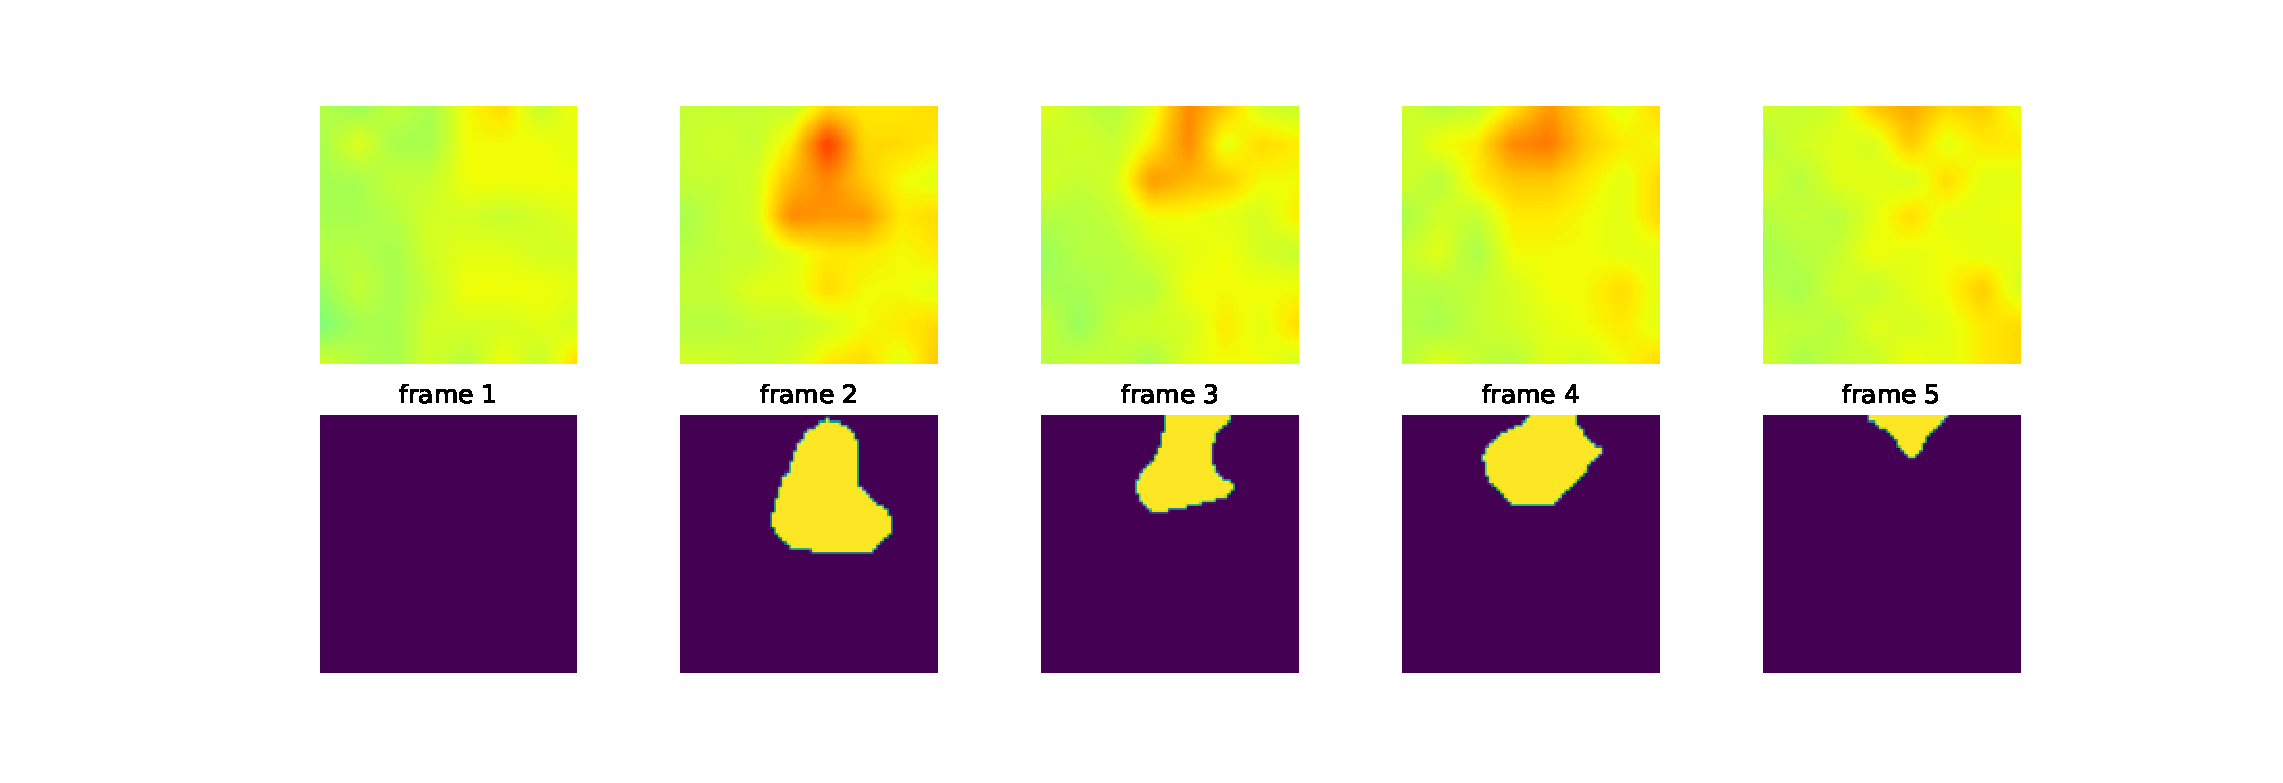
\includegraphics[width=\textwidth]{figures/err_missingframe.eps}
  \caption{This example shows an exit event where only the last few frames are captured, the missing frames of the event beginning makes it impossible to track and count the event correctly. The first row is the IR camera readings and the second row is the object mask.}\label{fig:err_mf}
\end{figure}
\autoref{fig:err_mf} demonstrates a typical detection failure that several beginning frames of an event are missed out. A further investigation shows this issue may be traced back to a network lagging. As mentioned in \Cref{ch:platform}, all the messages from the microcontroller are transmitted through a public MQTT broker so that realtime feedback can be obtained by running a listener client elsewhere. As contrary, in the controlled environment, both message publisher and listener locate under the same network and a local MQTT broker is used. Sending the messages to the Internet must have taken more time. Most of the message content is the raw IR image, which takes around 320 bytes. At a frame rate of 10 fps (when a human is detected), the generated data flow is about 3.5KB per second. Though the amount of data is still quite trivial, it is already larger than a common IoT application. Considering we use a public broker and the broker provider may have restrictions in the data amount, the network connection may deteriorate and finally cause a pause in the processing loop.

Moreover, the structure of the program could be improved. In the initial design, the message sending function is called within the tracking algorithm. Because it is observed that sending an image takes no longer than several milliseconds and will not break the time restriction for realtime processing. However, providing that a message sending may take several tens of milliseconds, the publishing task should be offloaded from the tracking algorithm. The task could be handled by another thread or even by the other CPU core. \autoref{fig:err_processloop} shows the improved program structure.
\begin{figure}
  \centering
    \subfloat[\centering the initial process loop]{{\includegraphics[width=0.3\textwidth]{figures/processloop1.png}}}%
    \qquad
    \subfloat[\centering the improved process loop]{{\includegraphics[width=0.6\textwidth]{figures/processloop2.png}}}%
    \caption{Initial and improved program flow. The orange blocks denote the time-consuming publishing tasks.}%
    \label{fig:err_processloop}
\end{figure}

After switching to a more stable broker, the number of missing frame error has reduced by 40\% (from 33 to 20). A lower error rate is expected when the publishing task is excluded from the process loop. Switching to a local broker instead of a public broker may also improve the network connection. Eventually, the image publishing task can be canceled totally because it is not needed in the deployment.

\subsection{Heat Disturbance Error}
\begin{figure}
  \centering
  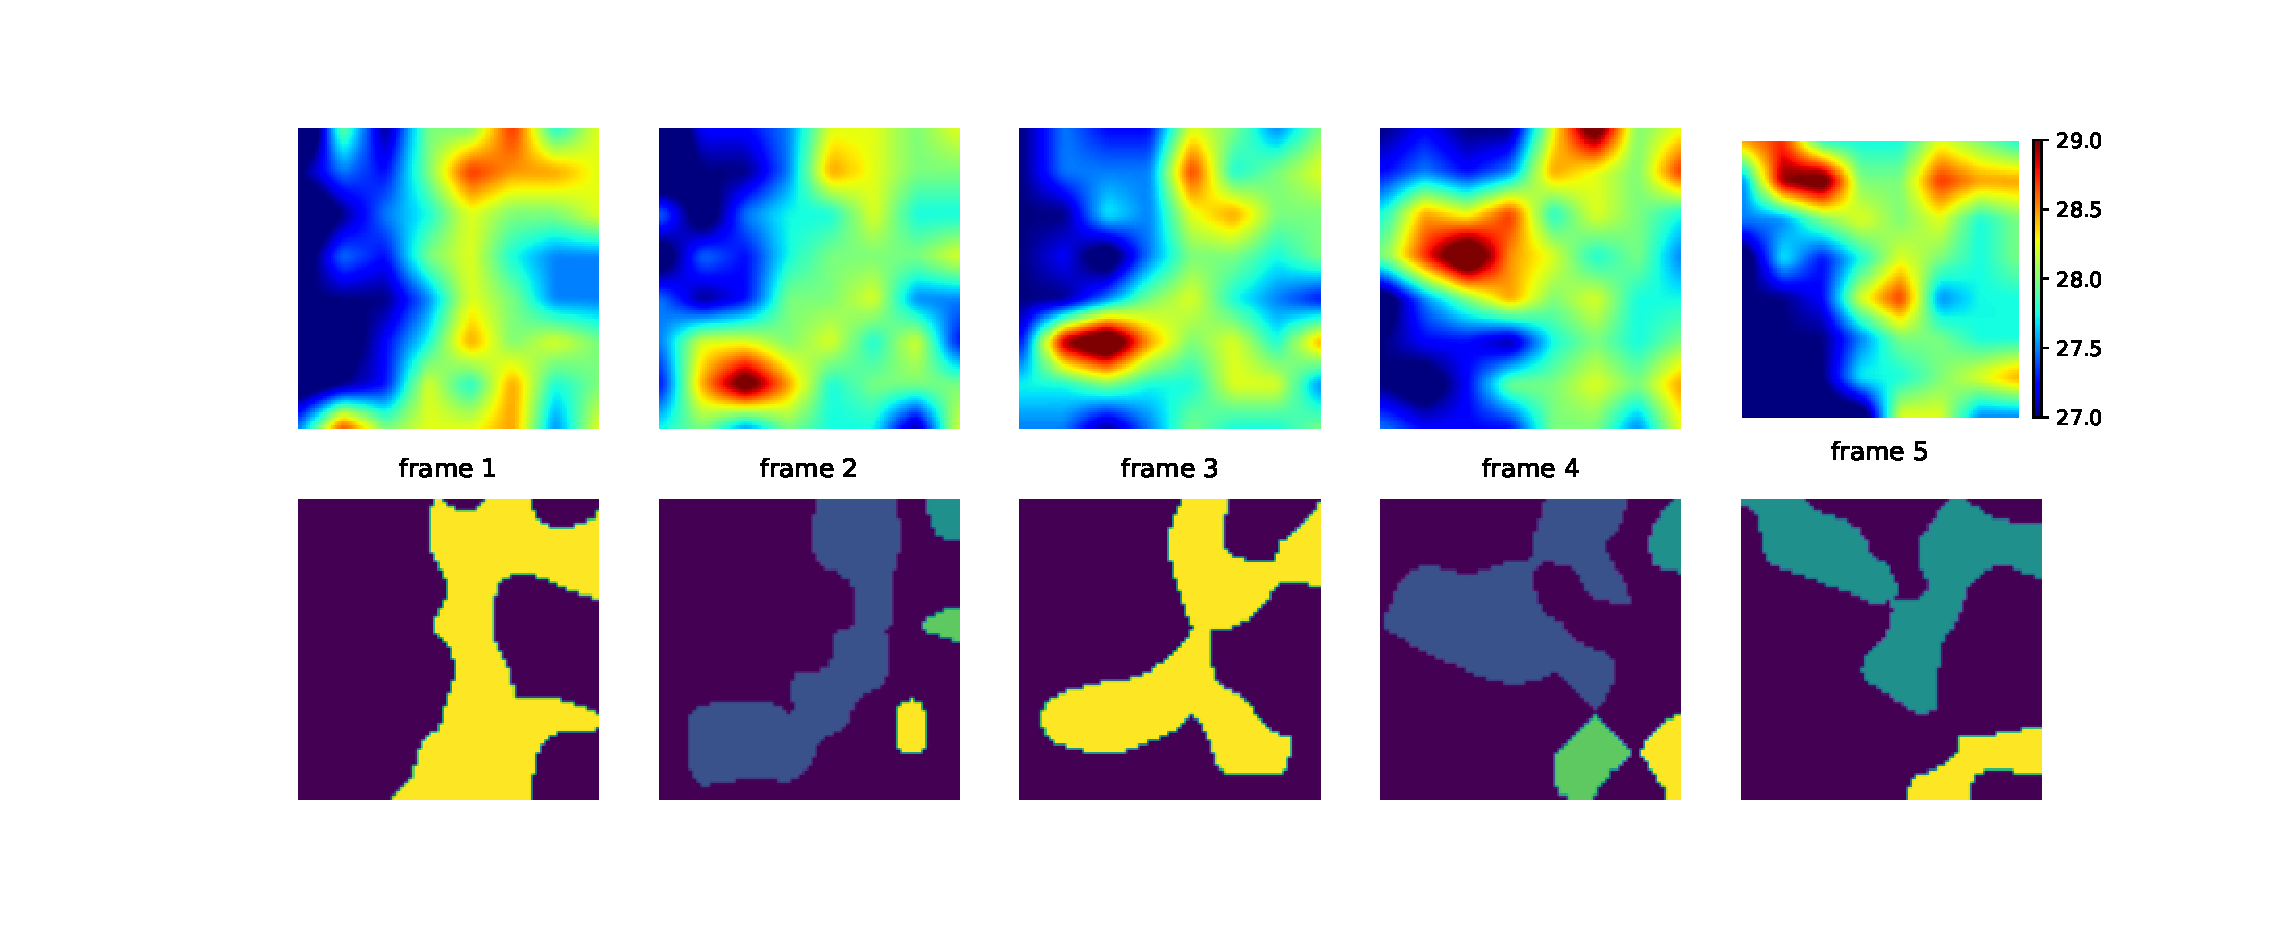
\includegraphics[width=\textwidth]{figures/err_heatdisturb.eps}
  \caption{This example shows a human leaving the room (on the left side), while half of the monitored area (on the right side) is heated up close to human body temperature. The first row is the IR camera readings and the second row is the erroneous object mask. The colorbar unit is $^\circ C$.}\label{fig:err_hd}
\end{figure}
Another frequent occurred abnormal scenario is the ``heat disturbance'' issue, where a constant heat source in the camera view interferes with the object detection procedure severely. A temperature rising in the partial background can be caused by a long time of exposure to the sunshine. A typical scenario is when only part of the floor is shined. For example, a doorway facing the direction of sunrise usually has its outer side shined and the inner side in the shadow. Several hours of sunshine is sufficient to cause a distinct temperature difference on different sides of the doorway. The developed algorithm holds the assumption that the background temperature is average within the whole camera view, and the background temperature is lower than the human body temperature. When this assumption does not hold anymore, human objects can no longer be segmented from the background. \autoref{fig:err_hd} shows that heat reflection from the ambient environment (floors, walls, etc.) can reach up to the human body temperature.

Moreover, the increased installation height has also contributed to the issue. Since the infrared ray emissivity attenuates by squared distance, the captured human body temperature becomes lower when the distance between the camera and the human increases (from 2 meters to 3 meters).

Overall, the heated ambient environment and a lower detected body temperature lead to a challenge in human object segmentation. And this segmentation challenge can not be solved by picking a well-selected threshold because the IR camera we used has an accuracy of $\pm 2.5^\circ C$. Therefore, we consider the heat disturbance issue as a hardware limit problem. A more precise segmentation should be achieved by switching to a better IR camera with higher precision.

\subsection{Other Errors and Anomalies}
\begin{figure}
  \centering
  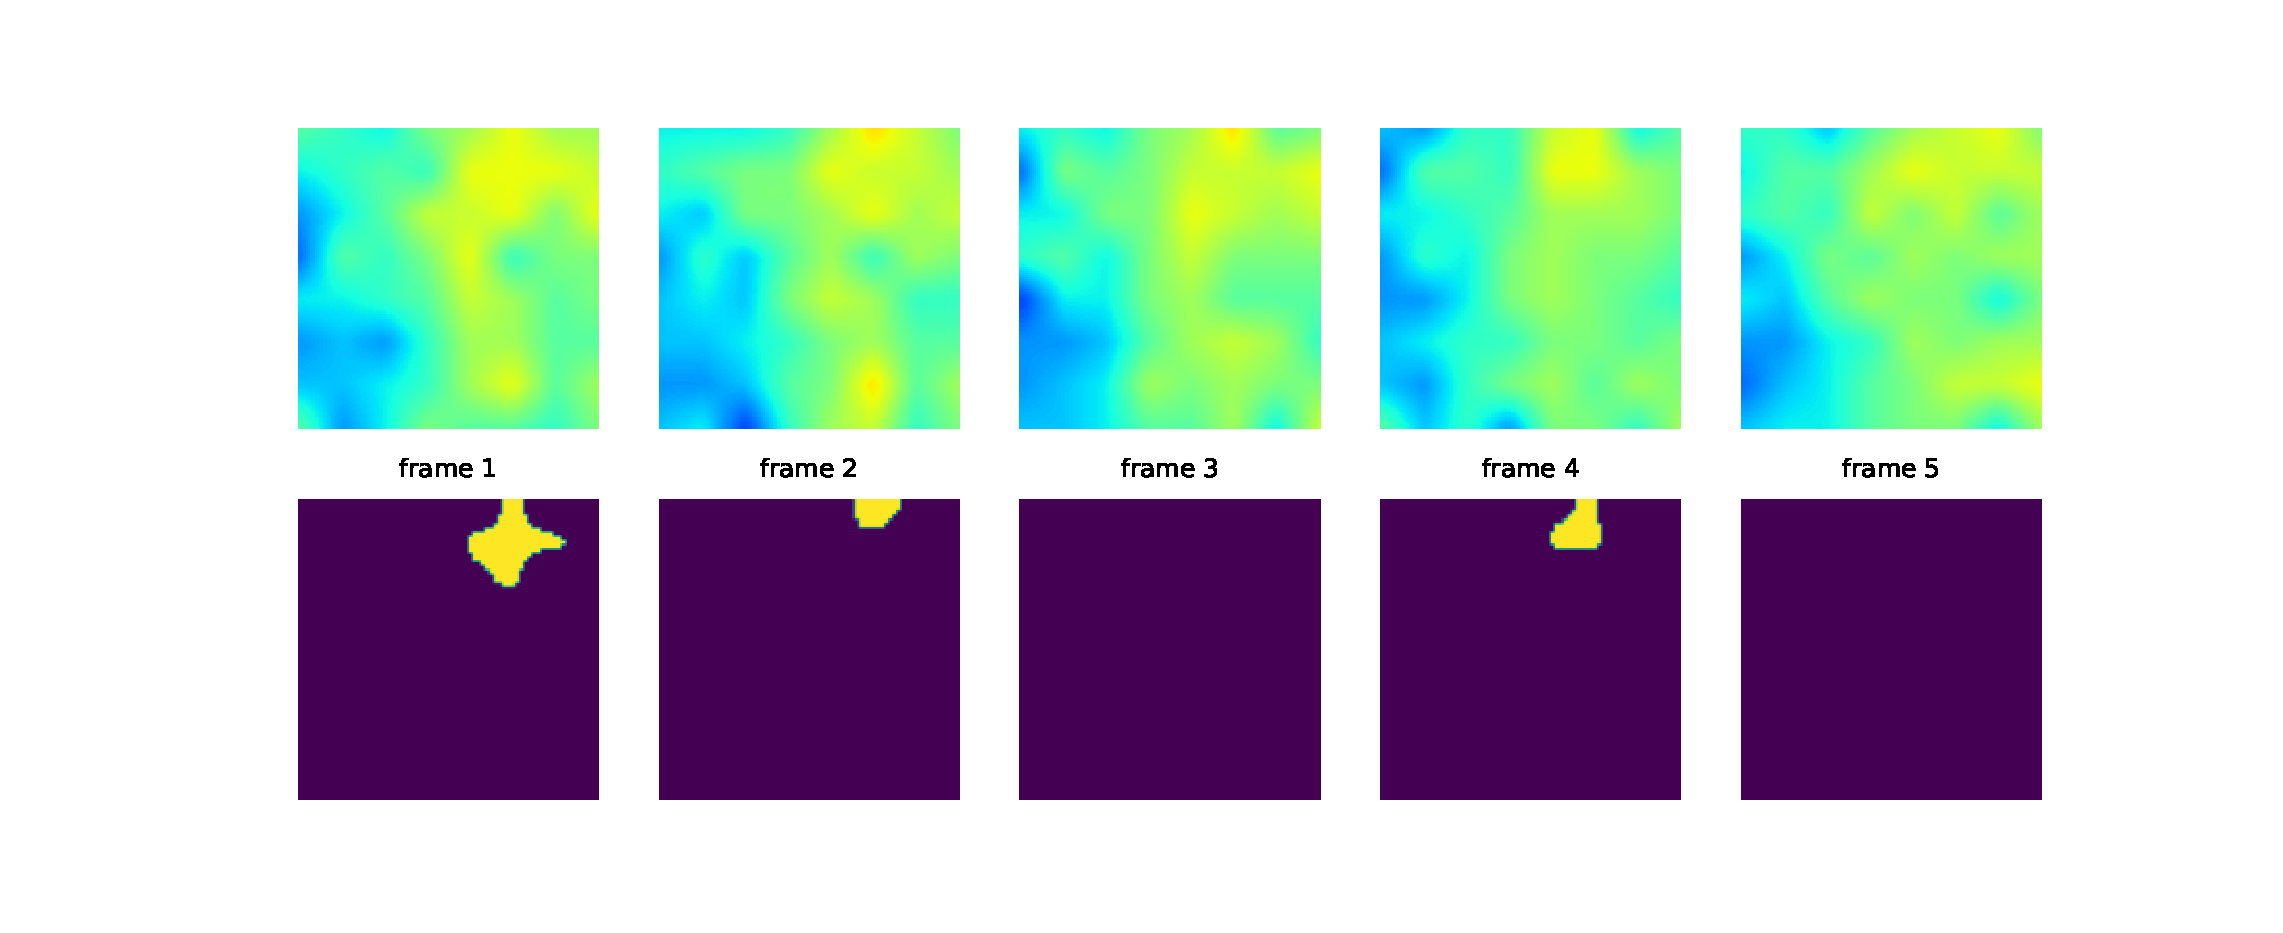
\includegraphics[width=\textwidth]{figures/err_noise1.eps}
  \caption{Sensor noises will not be tracked and counted even when they are incorrectly detected as objects because the sequence is usually not coherent.}\label{fig:err_no1}
\end{figure}
\begin{figure}
  \centering
  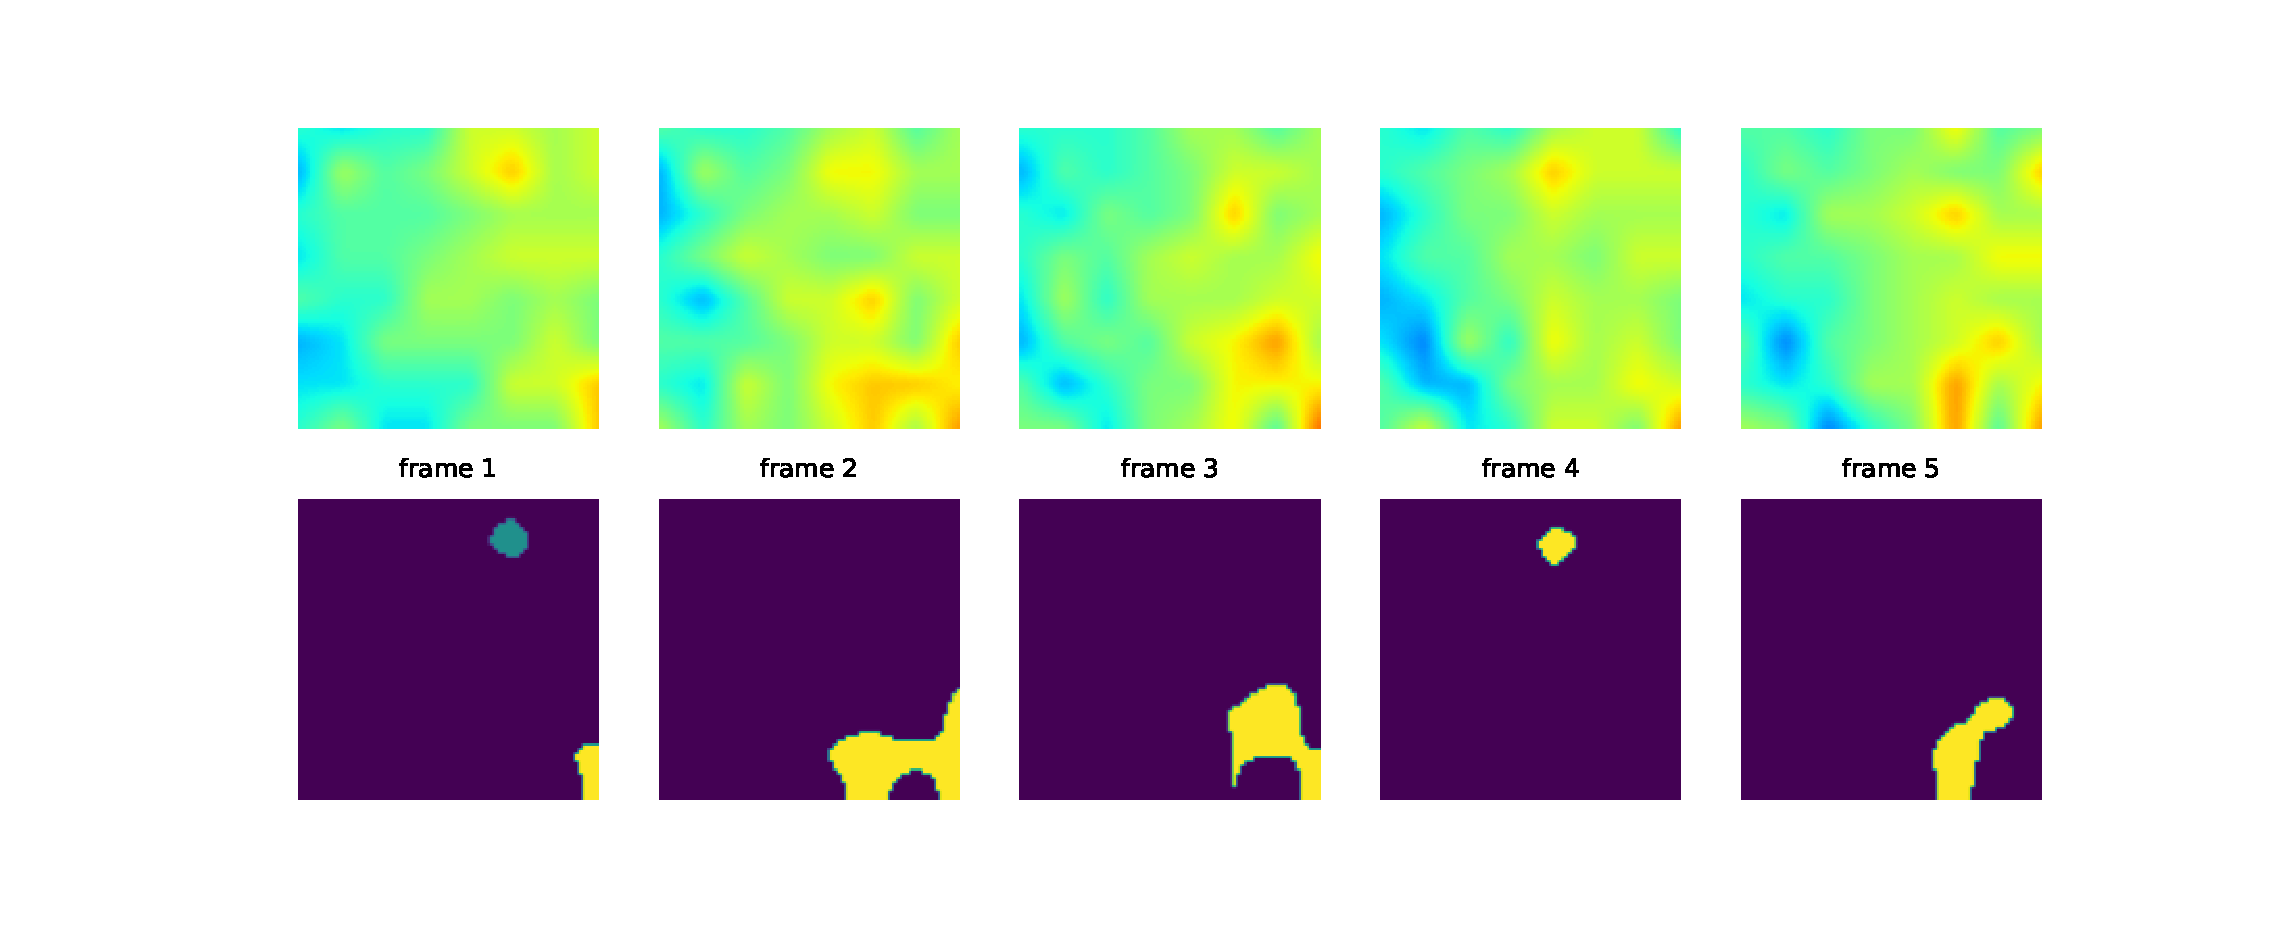
\includegraphics[width=\textwidth]{figures/err_noise2.eps}
  \caption{A noisy image sequence that may generate a wrong counting result. In the first 3 frames, the tracker has spawned an object in the right-bottom corner of the image. Later, the noise in frame 4 may be matched with the noise in frame 3, and the non-existing ``object'' has passed across the middle line. And in the next frame it disappears, which is considered as the termination of an exiting event. The human count is incorrectly decreased by one.}\label{fig:err_no2}
\end{figure}
Sometimes the temperature of a few pixels may temporarily exceed the segmentation threshold and be regarded as objects. The result is a few small objects emerging and disappearing randomly. We name this anomaly ``noise''. \autoref{fig:err_no1} shows an example of a noisy sequence. Fortunately, sensor noises usually will not cause a problem because they do not have an enter or exit tendency pattern as humans do. Tracking of a false detected noise pixel will fail within one or two frames and do not have an impact on the counting result. The only drawback is that the device will send too many rubbish messages to the storage platform if the camera is frequently activated by noises, which brings about the difficulty in debugging. Nevertheless, there are some noise sequences that cause a malfunction in the tracker, see \autoref{fig:err_no2}. When two noise trunks happen to emerge sequentially at different sides of the middle line, the tracking algorithm will take them as two frames of a moving object and generates incorrect results. Interestingly, we found that most of the problematic noisy sequences take place in the midnight when the ambient temperature drops. Therefore, the sensor noise issue should be traced back to the object detection layer. An improvement in \autoref{eq:detectionthreshold} may solve this problem.

Another potential issue takes place when a human stands under the camera for a long time, which is named as ``long sequence''. When there is an object in the camera view, the counting device needs to track it for every frame. The object must be segmented from the background over and over, the tracker needs to track the object even if it does not move at all, and the radio module keeps sending messages in minutes, which results in a lot of waste of computation power. Moreover, if a human occupies a certain area in the camera view, it increases the chance of incorrect matching when another person passes by. We have observed 6 long sequence anomalies during the real situation evaluation and all of them have been handled correctly.

Finally, the ``not detected'' issue describes when a human object passes under the camera but is not detected. This may happen when the human body temperature is too low, either because the body is covered by clothes or the person is short (the distance between camera and body enlarges for a short person, thus a lower detected body temperature). This issue can be solved by switching to a better IR camera with a larger detection range. It is also worth mentioning that the device only sends raw IR images for ground truth annotation when there are at least three pixels hotter than the room temperature. Therefore it is very likely that more events are not detected but also not noticed at all. This system bias in our experiment design can be solved by introducing another counting device based on different principles as a reference, for example, light barriers. An RGB camera may also help in collecting the ground truth if the privacy violation issue is lifted.

\section{Power Consumption}
The power consumption of the whole device is also an important aspect of the evaluation. The DHT11 temperature sensor consumes 1mA when measuring and 150µA when standby. The AMG8833 IR camera should run constantly and its average consumption is 4.5mA. \autoref{tab:esp32_power} shows the current consumption of the ESP32 in different modes. Without any power-saving tricks, the microcontroller consumes around 30mA (clock rate 160MHz) when idle and around 200mA when a human passes by. Assuming there are 40 enter and exit events every day and each event lasts 4 seconds (from image capturing until message publishing), the daily power consumption can be calculated approximately by \autoref{eq:power_estimate1}. On a common 600mAh Lipo battery, the device can operate for 16.5 hours, which is unsatisfying for an IoT application.
\begin{equation}\label{eq:power_estimate1}
\begin{split}
  P = (I_{esp32\ idle}+ I_{dht11}+I_{camera})mA * 24 hours + I_{esp32\ active}* t *n\\ \approx 852mAh +  9mAh = 860mAh
\end{split}
\end{equation}

It can be observed that though the radio module consumes the highest peak current, most of the battery power is wasted during the idle time because the device has to monitor the doorway all the time. To prolong the battery life, the key is how to reduce the power consumption when there is no event. Fortunately, Espressif provides many low-power options that can be integrated into our project. The light sleep mode can clock-gate the CPU and resume when an interrupt is triggered in the RTC peripheral. The deep sleep mode can power off the CPU totally to drastically reduce the power consumption lower than 1mA. Moreover, there is an 8MHz ultra-low-processor (ULP) along with the dual-core CPU that can retrieve sensor state and do some basic calculations when the main processors enter sleep mode, it can also wake up the main processors when necessary.

The power-saving design of our project contains two phases. The idle phase mainly contains the active pixel detection, i.e. the camera is polled by the ULP every 100ms to check if there is any pixel hotter than the environment temperature. And in the active phase, the ULP hands over the control of the camera to the main processors to track the object. To ensure an instant response of the human monitor device, we choose the light sleep mode because power up the main processors from deep sleep takes at least one second. Furthermore, we can neither afford the overhead of establishing the network connection whenever the main processor wakes up, so the RF module is kept powered on during sleep time. This results in power consumption of around 5mA during idle time. With the new idle current consumption, the daily consumption of the device is reduced to around 240mAh, and it can last around 2.5 days on a 600mAh battery.

More power is saved by deactivating the radio module so that the light sleep mode can be fully exploited. A constant network connection is required because the image data are too large to store in the internal memory, therefore we need to publish messages instantly. However, the image data are merely published for evaluation purpose and our algorithm works without the stored images. Without the image data, messages can be buffered in the memory and only send out once every hour. By this way we only bear the high current consumption during the relative short publish period and spare the expensive maintenance of the network. The estimated daily power consumption by this design is about 140mAh, see \autoref{eq:power_estimate2}. 
\begin{equation}\label{eq:power_estimate2}
\begin{split}
  P = (I_{esp32\ idle}+I_{camera})mA * 24 hours + I_{esp32\ active}* t_{event} *n \\+ I_{esp32\ publish}*t_{publish}*24\\ 
  \\\approx (1mA+ 4mA) * 24 hours + 40mA * (4s/3600) hours * 40 \\+ 180mA * 10s * 24
  \\= 120mAh +  8mAh + 12 = 140mAh
\end{split}
\end{equation}

By introducing additional sensors to detect approaching humans, the camera module no longer needs to operate constantly, which saves more power. For example, PIR sensors can be installed at both directions of the doorway to wake up the counting device in advance.   
The battery life can be further prolonged by deliberately shut down the device during midnight when it is unlikely to have any event.

\begin{table}[]
\centering
\begin{tabular}{|l|l|l|}
\hline
\textbf{Power mode}                  & \textbf{Description}            & \textbf{Power consumption} \\ \hline
Active (RF working)         & Wi-Fi transmit 802.11n & 180mA             \\
                            & Wi-Fi receive 802.11n  & 95 $\sim$100mA    \\ \hline
Active (RF not working)     & dual core 240MHz       & 30mA $\sim$68mA   \\
                            & dual core 160MHz       & 27mA $\sim$44mA   \\
                            & dual core 80MHz        & 20mA $\sim$31mA   \\ \hline
Light sleep with RF working & -                      & 5mA               \\
Light sleep                 & -                      & 0.8mA             \\ \hline
Deep sleep                  & ULP powered on         & 150µA             \\ \hline
\end{tabular}\caption{Power consumption of ESP32-WROVER module in different modes. The values are given by the ESP32 datasheet \cite{esp32datasheet} and confirmed by actual measurements.} \label{tab:esp32_power}
\end{table}

\section{Limitations}
The proposed algorithm has a few fundamental shortages. First of all, the object detection phase strongly depends on an accurate room temperature measurement and has a deterministic influence on the tracking result as the segmented object is the base of the following steps. Besides, the tracking algorithm based on central points can only handle multi-human events up to three or four people, if they were separated in the first few frames. The central point representation won't reflect the truth in crowded scenarios because multiple people will be regarded as one, for example, a large number of people crowding at the doorway when a meeting ends. Furthermore, our algorithm can not track a human who runs through the doorway, because the nearest neighbor matching method assumes the largest matching radius that is calculated from common walking speed.

There are also limitations to hardware. Currently, it takes around 20ms to process a single frame at a 160MHz CPU clock rate. The processing time may be longer if switching to a low-end MCU and eventually exceeds the time constraint. The program requires 953KB Flash and 220KB memory, the large memory requirement is mainly because of the image interpolation step. For images smaller than $71\times71$ resolution, the memory usage will likely remain the same. For larger images, both memory usage and process time will increase. 
\chapter{Conclusion and Future Works}
In this thesis, we have proposed a privacy-preserving human tracking algorithm, which receives top-view IR images as input and outputs the relative count of an enter or exit event at the doorway. The nature of low-resolution IR cameras prevents privacy violation fundamentally. We proposed to use a simple and effective segmentation threshold for object segmentation, use both centroids and central points to represent a binary blob, track the blob by nearest neighbor matching and finally filter the tracking result with an alpha-beta filter. The algorithm is capable to track single human passing through the doorway but also multiple humans at a common walking speed. We have deployed the algorithm on an ESP32-WROVER microcontroller and developed a doorway event counter that can operate independently for 2.5 days given the Wi-Fi infrastructure. The counted events are accumulated to obtain an estimation of building occupancy, which can be used in pandemic social distance regulation, HVAC optimization, and elder people caring.

Switching to a better IR camera that supports a longer detection range, higher resolution, and higher frame rate can enhance the algorithm accuracy as well as detect enter and exit events at various speeds. But the deployment cost will increase. Within the same hardware budget, a more complicated segmentation strategy has the largest potential to improve the counting result. The heat reflected from the surrounding environment poses a challenge in object segmentation and this should be taken into consideration in the development.
\backmatter
%\appendix{}
%\microtypesetup{protrusion=false}
% \glsaddall{} % add all defined terms to glossary, even if not referenced in text
% \printglossaries{} % TODO: uncomment if glossary needed
\listoffigures{}
\listoftables{}
\printbibliography{}

\end{document} 